\documentclass{mipt-thesis-ms}
% Следующие две строки нужны только для biblatex. Для inline-библиографии их следует убрать.
\usepackage{mipt-thesis-biblatex}
\addbibresource{example.bib}
\usepackage{booktabs}

% Подключение пакетов для алгоритмов
\usepackage{algorithm}
\usepackage{algpseudocode}


\title{Спектральные характеристики представлений в CNN и трансформерах}
\author{Шамигулов И.\,И.}
\supervisor{Калмыков Н.\,И.}
\referee{Номинаньный Н.\,Н.}       % требуется только для mipt-thesis-ms
\groupnum{М05-412г}
\faculty{Физтех-школа прикладной математики и информатики}
\department{Кафедра алгоритмов и технологий программирования}

\setlength{\parindent}{1.25cm}

% Локализация надписей
\floatname{algorithm}{Алгоритм}
\renewcommand{\algorithmicrequire}{\textbf{Вход:}}
\renewcommand{\algorithmicensure}{\textbf{Выход:}}
\setcounter{tocdepth}{1}
\begin{document}

\titlepage \addemptypage

\newpage
\thispagestyle{plain}      % номер внизу по центру (если нужен)

\chapter*{Аннотация}       % или \chapter*{Аннотация}, если хотите без номера
Работа посвящена исследованию спектральных характеристик внутренних представлений моделей компьютерного зрения: свёрточных сетей ResNet, визуальных трансформеров ViT и иерархических трансформеров Swin. Цель исследования — количественно описать, как по мере углубления модели меняется распределение энергии представлений по пространственным частотам, и сравнить динамику между CNN и Transformer архитектурами.

В работе реализован единый протокол спектрального анализа. Для ResNet анализировались выходы основных блоков, для ViT и Swin последовательности токенов преобразовывались в двумерную решётку патчей. Для выбранных уровней выполнялись вычитание пространственного среднего, ДПФ, спектр мощности, усреднение по батчу и каналам и радиальное усреднение. Для сравнения использовались спектральный центроид, доля низких частот и скорость сжатия.

Эксперименты показали, что ResNet смещает представления к низким частотам: центроид уменьшается, а доля низкочастотной энергии возрастает. ViT имеет немонотонную динамику: в ряде моделей центроид на средних и поздних блоках не снижается, а возрастает. Swin занимает промежуточное положение: его иерархия приводит к низкочастотному финальному представлению, но сжатие спектра менее резкое, чем в CNN.

Результаты показывают, что тип архитектуры сильнее влияет на спектральную динамику, чем глубина внутри одного семейства. Подход может использоваться для диагностики моделей, особенно в задачах, чувствительных к деталям и локальным структурам.

\newpage
\tableofcontents % содержание
\pagestyle{miptthesis}

\chapter{Введение}

Современное компьютерное зрение развивается не только за счёт увеличения размеров датасетов и вычислительных ресурсов, но и за счёт усложнения архитектур нейронных сетей. За последние годы в этой области сформировались несколько крупных архитектурных направлений. Сначала основную роль играли свёрточные нейронные сети, затем широкое распространение получили глубокие остаточные модели ResNet, а позже в задачах зрения стали активно использоваться визуальные трансформеры и гибридные иерархические архитектуры Swin Transformer. Все эти модели достигали высокой точности на задачах классификации изображений. Но точность не объясняет, что именно происходит внутри модели. Две архитектуры могут давать близкий результат, но приходить к нему через разные внутренние признаки.

В прикладной постановке нейронную сеть часто воспринимают довольно просто: на вход подаётся изображение, на выходе получается класс. Для инженерного использования этого обычно хватает. Для исследовательской задачи — уже нет. Между входом и финальным ответом находится цепочка промежуточных представлений, и каждый уровень этой цепочки меняет исходный сигнал. Ранние слои, согласно тому как устроен CNN, обычно ближе к локальным деталям: границам, текстурам, цветовым переходам. Глубокие уровни работают уже с более собранными признаками — частями объектов, формой, семантическими структурами. Поэтому в данной работе рассматривается не только финальное предсказание, но и то, как меняется само представление изображения по глубине модели.

Одним из способов такого анализа является изучение представлений в частотной области. Изображение можно рассматривать как сигнал, состоящий из компонент разного масштаба. Низкие пространственные частоты соответствуют плавным изменениям яркости, крупным областям и общей форме объекта. Высокие пространственные частоты связаны с резкими переходами, границами, текстурами, мелкими деталями и шумовыми компонентами. Если применить такую точку зрения не только к исходному изображению, но и к промежуточным представлениям нейронной сети, появляется возможность исследовать, какие частотные компоненты сохраняются, подавляются или перераспределяются по мере углубления модели.

Для свёрточных нейронных сетей такая постановка выглядит естественной. Внутренние представления CNN имеют форму двумерных карт признаков, то есть сохраняют пространственную структуру изображения. Кроме того, сама операция свёртки имеет тесную связь с частотной областью: фильтр может усиливать или подавлять различные частотные компоненты сигнала. При этом классические CNN обычно строят иерархию признаков: пространственное разрешение карт постепенно уменьшается, число каналов растёт, а рецептивное поле становится шире. Поэтому можно ожидать, что по мере углубления свёрточной сети высокочастотные локальные детали будут постепенно уступать место более низкочастотным и семантически обобщённым признакам.

Архитектуры ResNet являются одним из наиболее важных представителей CNN-семейства. Их ключевая особенность — остаточные связи, позволяющие эффективно обучать глубокие сети и уменьшать проблему деградации качества при увеличении числа слоёв \cite{he2016deep}. Благодаря этому ResNet удобно использовать для анализа влияния глубины на внутренние представления: в одном семействе можно сравнивать модели разного масштаба, такие как ResNet18, ResNet34, ResNet50 и ResNet101. В данной работе ResNet рассматривается как базовый пример иерархической свёрточной архитектуры.

Визуальные трансформеры устроены принципиально иначе. Vision Transformer разбивает изображение на непересекающиеся патчи, преобразует каждый патч в токен и далее обрабатывает последовательность токенов с помощью блоков самовнимания \cite{dosovitskiy2021image}. Эта идея основана на архитектуре Transformer, изначально предложенной для обработки последовательностей \cite{vaswani2017attention}. В отличие от CNN, ViT не использует явную свёрточную локальность и не строит пространственную иерархию тем же способом. Из-за этого возникает важный вопрос: будет ли ViT демонстрировать ту же частотную динамику, что и CNN, или механизм внимания приводит к иному перераспределению спектральной энергии?

Этот вопрос становится особенно важным на фоне исследований, показывающих, что визуальные трансформеры отличаются от CNN не только архитектурно, но и по характеру внутренних представлений. Например, в работе \cite{raghu2021do} показано, что ViT и CNN по-разному агрегируют пространственную информацию и формируют признаки по глубине. Исследование \cite{park2022how} рассматривает механизм самовнимания как оператор, обладающий низкочастотными свойствами, однако из этого не следует автоматически, что все внутренние представления ViT должны монотонно сжиматься к низким частотам. На итоговый спектр влияет не только attention, но и остаточные связи, нормализации, MLP-блоки, позиционные эмбеддинги и способ организации токенов.

Swin Transformer занимает в этом сравнении отдельное место. Его нельзя отнести ни к классическим свёрточным сетям, ни к обычному ViT без оговорок. От трансформеров Swin наследует токенное представление и механизм внимания, а от CNN — многоуровневую обработку с уменьшением пространственного разрешения. В архитектуре это реализуется через оконное внимание, сдвиг окон между соседними блоками и объединение патчей \cite{liu2021swin}. Поэтому Swin удобен как промежуточный объект анализа: на нём можно отдельно посмотреть, как локальность, иерархия и attention-механизм связаны с частотным составом признаков. Сравнение ResNet, ViT и Swin в этой работе фактически сводится к сравнению трёх способов обработки изображения: свёрточной пирамиды, глобальной токенной модели и локально-иерархического трансформера.

Мотивация работы связана с простой проблемой: accuracy показывает качество ответа, но почти ничего не говорит о том, за счёт каких признаков этот ответ был получен. Модели с близкой точностью могут по-разному реагировать на шум, изменение текстуры, доменный сдвиг или потерю мелких деталей. Частотный анализ даёт здесь дополнительный язык описания. Через него можно увидеть, сохраняет ли представление вклад локальных изменений или быстро переходит к более сглаженной структуре. Для задач медицинской визуализации, спутниковых снимков, дефектоскопии, текстур и мелких объектов это не абстрактный вопрос: слишком раннее подавление высоких частот может убрать признаки, которые несут полезную информацию. В более прикладном смысле такие наблюдения могут пригодиться при регуляризации, дистилляции, сжатии моделей и анализе устойчивости к возмущениям.

Теоретическая опора исследования — работы о spectral bias, то есть о частотном смещении нейронных сетей. В \cite{rahaman2019spectral} показано, что сети обычно быстрее осваивают низкочастотные компоненты функций, а более резкие, высокочастотные зависимости требуют большего усилия при обучении. Позднее эта линия была развита в исследованиях frequency principle и формальных способов измерения спектрального смещения \cite{xu2025overview,kiessling2022computable}. Для компьютерного зрения есть и отдельная мотивация: высокочастотные компоненты изображений связывают как с обобщающей способностью, так и с робастностью моделей \cite{yin2019fourier,wang2020highfrequency}. В этой работе такие результаты используются не как прямой предмет проверки, а как основание для анализа: если частоты влияют на поведение модели, то спектр внутренних представлений может многое сказать о том, какие признаки сохраняются по мере прохождения изображения через сеть.

При этом в существующей литературе разные стороны этой проблемы чаще изучаются раздельно. Одни работы рассматривают общие свойства spectral bias и роль частотных компонент в обучении нейронных сетей. Другие анализируют связь частот с робастностью и обобщением CNN \cite{yin2019fourier,wang2020highfrequency}. Отдельное направление посвящено визуальным трансформерам: их механизму внимания, устойчивости и использованию высокочастотной информации \cite{park2022how,bai2022improving,naseer2021intriguing,paul2022vision}. Однако для сравнения CNN, ViT и Swin требуется единая экспериментальная постановка, в которой разные архитектуры анализируются по одним и тем же спектральным характеристикам. Именно эту задачу решает данная работа: она строит общий протокол анализа представлений и позволяет сопоставить частотную динамику трёх архитектурных семейств на единой основе.

Цель данной выпускной квалификационной работы — исследовать спектральные характеристики внутренних представлений CNN и визуальных трансформеров разной архитектуры и глубины, а также определить, как тип архитектуры влияет на распределение спектральной энергии по слоям.

Для достижения поставленной цели были сформулированы следующие задачи:

\begin{enumerate}
\item изучить теоретические основы спектрального анализа нейросетевых представлений и связанные исследования по spectral bias, CNN и визуальным трансформерам;
\item описать архитектурные особенности ResNet, ViT и Swin, влияющие на пространственную и частотную структуру признаков;
\item реализовать единый экспериментальный протокол извлечения промежуточных представлений из моделей разных архитектур;
\item адаптировать спектральный анализ к токенным представлениям ViT и Swin через восстановление двумерной решётки патчей;
\item построить радиальные спектральные кривые для выбранных уровней ResNet, ViT и Swin;
\item рассчитать количественные метрики спектральной динамики: спектральный центроид, долю низкочастотной энергии и скорость спектрального сжатия;
\item сравнить спектральную динамику внутри каждого архитектурного семейства и между семействами ResNet, ViT и Swin;
\item сопоставить спектральные характеристики с точностью классификации и сформулировать выводы о связи между архитектурой, спектральным профилем и качеством модели.
\end{enumerate}

Объектом исследования являются внутренние представления моделей компьютерного зрения. Предметом исследования являются спектральные характеристики этих представлений: распределение энергии по пространственным частотам, изменение частотного профиля по глубине модели и различия между архитектурными семействами.

В качестве экспериментальных объектов рассматриваются три семейства моделей. Семейство ResNet используется как представитель свёрточных архитектур. Семейство Vision Transformer используется как представитель моделей, основанных на глобальной обработке последовательности патчей. Семейство Swin Transformer используется как представитель иерархических трансформеров с локальным оконным вниманием. Эксперименты проводятся на изображениях из набора ImageNet, который является стандартным датасетом для оценки моделей компьютерного зрения \cite{deng2009imagenet}. В практической части используется подвыборка ImageNet 10K \cite{priyerana_imagenet10k}.

В работе были сформулированы четыре исследовательские гипотезы.

Первая гипотеза состоит в том, что в свёрточных сетях семейства ResNet по мере углубления модели происходит устойчивое спектральное сжатие. Иными словами, ожидается снижение спектрального центроида и рост доли низкочастотной энергии от ранних слоёв к глубоким.

Вторая гипотеза состоит в том, что Vision Transformer не должен полностью повторять монотонную низкочастотную динамику CNN. Поскольку ViT работает с последовательностью патчей и использует самовнимание, MLP-блоки, нормализации и остаточные связи, его спектральная динамика может быть немонотонной.

Третья гипотеза состоит в том, что Swin Transformer должен занимать промежуточное положение между CNN и ViT. За счёт иерархической структуры и patch merging он должен приходить к более низкочастотным финальным представлениям, однако на промежуточных блоках возможна более сложная динамика, чем у классической CNN.

Четвёртая гипотеза состоит в том, что спектральные метрики не должны иметь простой линейной связи с точностью классификации. Они отражают характер внутренних представлений, но не являются самостоятельной заменой accuracy и других метрик качества.

Научная новизна работы заключается в применении единого протокола спектрального анализа к архитектурам различной природы: свёрточным сетям, визуальным трансформерам и иерархическим трансформерам. В отличие от исследований, сосредоточенных только на CNN или только на механизме внимания, в данной работе проводится сопоставление трёх архитектурных семейств на одной методологической основе.

Практическая значимость работы состоит в том, что предложенный подход может использоваться как инструмент диагностики моделей компьютерного зрения. Он позволяет оценивать, насколько быстро модель теряет или сохраняет частотное разнообразие признаков. Это может быть полезно при выборе архитектуры для задач, чувствительных к локальным деталям, а также при разработке методов регуляризации, дистилляции и повышения устойчивости моделей.

Структура работы организована следующим образом. В первой главе формулируются актуальность, цель, задачи, объект, предмет и гипотезы исследования. Во второй главе рассматриваются теоретические основы: понятие внутренних представлений, спектральный анализ, частотные свойства изображений, CNN, ResNet, ViT, Swin и связанные исследования. В третьей главе описывается методика эксперимента: извлечение представлений, построение спектральных кривых и расчёт метрик. В четвёртой главе приводятся результаты экспериментов и их интерпретация. В заключении формулируются основные выводы, ограничения работы и направления дальнейших исследований.

\chapter{Теоретические сведения}

Данная глава вводит основные понятия, необходимые для понимания методики и результатов работы. В ней рассматриваются внутренние представления нейронных сетей, частотный анализ изображений, свойства спектра, архитектуры ResNet, Vision Transformer и Swin Transformer, а также исследования, связывающие частотные характеристики с обучением и интерпретируемостью моделей компьютерного зрения.

\section{Внутренние представления и частотная интерпретация}

\subsection{Внутренние представления моделей компьютерного зрения}

Глубокую нейронную сеть можно рассматривать как последовательность преобразований входных данных. В случае компьютерного зрения на вход модели подаётся изображение, а на выходе получается предсказание: например, класс объекта. Однако между входом и выходом находится большое число промежуточных слоёв. Каждый слой преобразует данные в новую форму. Эти промежуточные результаты называются внутренними представлениями, признаками или активациями.

Интуитивно внутреннее представление — это то, как сама модель «видит» изображение на некотором этапе обработки. На ранних слоях признаки обычно ближе к исходному изображению: они могут реагировать на границы, контуры, простые текстуры и локальные цветовые переходы. На более глубоких слоях признаки становятся более абстрактными: отдельные нейроны или каналы могут реагировать уже не на конкретный пиксельный рисунок, а на части объектов, повторяющиеся структуры или семантические категории. Такая иерархия признаков является одной из причин эффективности глубоких моделей.

Для свёрточных сетей внутренние представления обычно имеют вид карт признаков. Карта признаков — это двумерная сетка значений, похожая на изображение, но вместо исходных пикселей она содержит отклики фильтров. Если у изображения есть три канала цвета, то у карты признаков глубокого слоя могут быть десятки, сотни или тысячи каналов. Каждый канал можно понимать как отдельный тип признака, который модель научилась выделять.

Для трансформеров представления имеют другую форму. Визуальный трансформер разбивает изображение на патчи, то есть небольшие непересекающиеся фрагменты. Каждый патч превращается в вектор — токен. После этого модель работает не с изображением как с двумерной сеткой пикселей, а с последовательностью токенов. Поэтому анализ трансформеров требует дополнительной интерпретации: чтобы сравнить их с CNN, токены можно вернуть в двумерную решётку, соответствующую расположению патчей в исходном изображении.

Внутренние представления важны, потому что именно они определяют поведение модели. Две архитектуры могут иметь похожую точность классификации, но при этом строить совершенно разные признаки. Одна модель может сильнее опираться на текстуры, другая — на форму объекта, третья — на глобальный контекст. Поэтому анализ внутренних представлений позволяет лучше понять, почему модель работает именно так, как она работает.

Классическая работа \cite{yosinski2014transferable} показывает, что признаки разных уровней обладают разной степенью переносимости между задачами. Ранние признаки часто оказываются более универсальными, тогда как поздние сильнее связаны с конкретной задачей и датасетом. В данной работе этот взгляд дополняется частотной интерпретацией: нас интересует не только то, насколько признаки переносимы, но и то, как по глубине модели меняется их спектральный состав.

\subsection{Изображение как пространственный сигнал}

Для понимания спектрального анализа важно рассматривать изображение не только как набор пикселей, но и как пространственный сигнал. Пространственный сигнал — это функция, которая задана на координатной сетке. В каждой точке изображения есть соответствующее значение цвета или яркости, в зависимости от используемой цветовой модели. 
При движении по координатной сетке может быть плавное и медленное изменение значения от пикселя к пикселю, а может резко изменяться - первое поведение соответствует низким пространственным частотам, второе - высоким пространственным частотам.

Плавный фон, большое однотонное пятно, объект крупной формы - все это пример низкочастотной структуры. Резкие границы, тонкие линии, мелкие детали и текстуры и шум - высокочастотная структура. Реальное изображении содержит в себе одновременно компоненты разных частот. Например, фотография собаки на заднем сиденье содержит низкочастотную информацию о силуэте и общей форме животного и фона, высокочастотную информацию о шерсти, краях и мелких деталях.

Для решения задач компьютерного зрения важно это учитывать. Для одних задач достаточно низких частот: например, чтобы грубо отличить автомобиль от самолёта, часто хватает общей формы. Для других задач высокие частоты критичны: в медицинских снимках, спутниковых изображениях или дефектоскопии мелкие детали могут нести ключевую информацию. Поэтому способность модели сохранять или подавлять разные частотные компоненты влияет на её применимость к конкретным задачам.

Частотный анализ позволяет перейти от вопроса «какие значения имеют пиксели или активации?» к вопросу «какие масштабы изменений представлены в сигнале?». В этой работе такой подход применяется не только к исходным изображениям, но и к промежуточным представлениям нейронных сетей.

\subsection{Спектр, частотный радиус и радиальное усреднение}

Спектр — это описание сигнала через набор частотных компонент. В пространственной области мы смотрим, как значения сигнала расположены по координатам. В частотной области мы смотрим, из каких колебаний разного масштаба этот сигнал состоит. Можно сказать, что спектр показывает, сколько в сигнале «медленных» и «быстрых» изменений.

Для изображения низкие частоты отвечают за крупные и плавные структуры. Средние частоты часто связаны с частями объектов, локальными формами и выраженными, но не слишком мелкими деталями. Высокие частоты отвечают за резкие изменения, мелкие текстуры, тонкие контуры и шум. Поэтому спектр изображения можно использовать как способ описать, насколько изображение или карта признаков являются гладкими, детальными или шумными.

В спектральном анализе обычно различают амплитуду, фазу и энергию. Амплитуда показывает силу частотной компоненты. Фаза содержит информацию о расположении соответствующей структуры в пространстве. Энергия показывает вклад частоты в общий сигнал. В данной работе, поскольку задача состоит в том, чтобы понять, какие частотные диапазоны сохраняются в представлениях разных слоёв, основной интерес представляет распределение энергии по частотам.

Также важной составляющей любого изображения является нулевая частота или, так называемая, DC-компонента. нулевая частота -  это постоянная составляющая сигнала, то есть его средний уровень. DC-компонента может оказаться очень большой и скрыть более содержательные различия между частотами, если среднее значение карты признаков имеет большое положительное значение. Поэтому в практическом анализе часто удаляют пространственное среднее перед вычислением спектра. Процедура этого шага подробно описана в главе с методикой работы.

По одному только спектру нельзя решить, полезна ли конкретная частота для классификации. Высокочастотная область может соответствовать границам и мелким деталям, но там же могут находиться шумовые или нестабильные компоненты. Низкие частоты часто отражают форму и крупные структуры, однако для некоторых задач такого описания слишком мало. Поэтому спектральный анализ в данной работе используется как способ описать представления, а не как самостоятельная мера качества модели

Изучение двухмерных карт признаков или изображений предполагает использование пространственного спектра с аналогичной размерностью. В двумерном спектре фиксируется амплитуда колебаний и направление: вертикальное, горизонтальное, диагональное и другие. Например, вертикальные и горизонтальные переходы могут характеризоваться сопоставимым пространственным масштабом, но различаться по ориентации в частотной плоскости. 

Направление не имеет значения, поэтому для анализа важен лишь частотный масштаб, из-за чего исходный двумерный спектр преобразуется в радиальную одномерную кривую. Для этого частоты с одинаковым расстоянием от центра спектра усредняются. Получается зависимость энергии от частотного радиуса. Малый радиус соответствует низким частотам, большой радиус — высоким.

Радиальный спектр удобен для сравнения разных моделей и слоёв. Вместо сложной двумерной карты мы получаем одну кривую, по форме которой можно судить о частотном профиле представления. Если кривая быстро убывает после пика в низких частотах, значит представление сильно сконцентрировано в низкочастотной области. Если хвост кривой тянется дальше, значит в представлении сохраняется вклад средних или высоких частот.

В результатах работы используется нормализованный частотный радиус. Это нужно для того, чтобы сравнивать слои с разным пространственным разрешением. Например, ранний слой CNN может иметь большую карту признаков, а поздний — маленькую. У таких карт различается максимальная представимая частота. Нормализация частотной оси позволяет привести кривые к сопоставимому виду. В экспериментальной части дополнительно используется приведение частотной шкалы к масштабу первого слоя, что позволяет сравнивать спектры разных блоков на общей оси.

\subsection{Интерпретация низких и высоких частот}

Спектральный анализ даёт удобный способ описывать внутренние представления модели, но трактовать его результаты нужно аккуратно. Прежде всего, спектральная энергия не является информацией в строгом теоретико-информационном смысле. Она показывает, как распределены активации по частотным диапазонам, но сама по себе не отвечает на вопрос, насколько эти признаки полезны для распознавания объекта.

То же относится и к разделению частот на низкие и высокие. Высокочастотная область может содержать действительно важные детали: границы, мелкие текстуры, локальные различия между объектами. Но в эту же область часто попадают шумовые и нестабильные компоненты. С низкими частотами ситуация похожая. Они могут хорошо передавать общую форму и крупную структуру объекта, однако для задач, где решающими оказываются небольшие отличия, такого описания может быть недостаточно. Поэтому в работе частотный профиль рассматривается не как прямой показатель качества, а как дополнительная характеристика представлений.

Отдельная осторожность нужна при сравнении CNN и трансформеров. Карта признаков свёрточной сети и решётка токенов ViT устроены по-разному. В CNN пространственные карты формируются последовательностью свёрточных фильтров. В ViT каждый токен соответствует целому патчу и уже содержит агрегированную информацию о фрагменте изображения. Возврат токенов к двумерной решётке позволяет применить общий спектральный аппарат, но не делает представления этих архитектур полностью одинаковыми.

Есть и ещё одно ограничение. В данной работе анализируются уже обученные модели, то есть фиксируется состояние представлений после завершения обучения. По таким данным можно сравнить финальную спектральную структуру слоёв, но нельзя проследить, как она возникала по эпохам. Для этого потребовался бы отдельный эксперимент: сохранять промежуточные состояния модели во время обучения и анализировать, как меняются спектральные характеристики на разных этапах.

В обычной обработке изображений низкие частоты часто связывают с общей формой и плавными областями, а высокие — с деталями и текстурами. В нейронных сетях эта интерпретация сохраняется, но становится более сложной. Внутренние представления — это уже не исходные пиксели, а признаки, сформированные моделью. Поэтому низкие частоты в карте признаков означают не просто плавность исходного изображения, а пространственную гладкость некоторого признака. Высокие частоты означают, что признак быстро меняется по пространственным координатам.

Например, если некоторый канал карты признаков активируется на всей области объекта, его спектр будет более низкочастотным. Если канал активируется только на узких границах или мелких деталях, в нём будет больше высокочастотных компонент. Если глубокий слой теряет высокочастотные компоненты, это может означать, что модель переходит от локальных деталей к более глобальным и устойчивым признакам. Но это также может означать потерю информации, важной для задач, чувствительных к мелким структурам.

Именно поэтому в данной работе используется термин «спектральная энергия представления». Он не означает информацию в строгом смысле теории информации Шеннона. Речь идёт о том, как энергия активаций распределена по пространственным частотам. Такой подход позволяет исследовать частотное разнообразие признаков, но не утверждает напрямую, что одна частота «важнее» другой для классификации.

Изменение частотного состава по глубине сети можно рассматривать как один из признаков того, как модель переходит от локальной информации к более обобщённым признакам.

В литературе показано, что частотные компоненты изображения могут быть связаны с поведением моделей компьютерного зрения. Например, в работе \cite{yin2019fourier} частотная область используется для анализа устойчивости моделей к различным искажениям, а в \cite{wang2020highfrequency} обсуждается роль высокочастотных компонент в обобщающей способности CNN. Эти результаты важны для данной работы не как непосредственный объект проверки, а как дополнительное обоснование того, что частотный состав представлений может отражать существенные свойства модели.

Для визуальных трансформеров вопрос частотной интерпретации также остаётся актуальным. Работы \cite{naseer2021intriguing,paul2022vision,alijani2024vision} показывают, что ViT могут отличаться от CNN по характеру устойчивости и внутренней организации признаков. Это согласуется с общей мотивацией настоящего исследования: сравнивать архитектуры следует не только по итоговой точности, но и по тому, как они преобразуют признаки внутри модели.


\section{Архитектуры компьютерного зрения}

\subsection{Свёрточные нейронные сети и ResNet}

Свёрточная нейронная сеть — это архитектура, специально приспособленная для обработки данных с пространственной структурой. В изображении соседние пиксели обычно связаны друг с другом, и CNN использует это свойство через локальные фильтры. Фильтр смотрит на небольшой участок изображения или карты признаков и вычисляет отклик. Один и тот же фильтр применяется во всех пространственных позициях, поэтому сеть может находить один и тот же признак в разных местах изображения.

Для понимания CNN важны несколько терминов. Канал — это отдельная карта признаков, соответствующая одному типу выделенного паттерна. Ядро свёртки — это небольшой набор весов, который перемещается по изображению. Stride — шаг, с которым фильтр проходит по пространственным координатам. Если шаг больше единицы, пространственное разрешение уменьшается. Pooling — операция агрегирования соседних значений, также часто уменьшающая разрешение. Рецептивное поле — область исходного изображения, которая влияет на конкретное значение в карте признаков. Чем глубже слой, тем больше обычно его рецептивное поле.

С точки зрения спектрального анализа CNN можно понимать как систему фильтров. Ранние фильтры часто реагируют на простые локальные структуры: границы, углы, текстуры. Такие признаки могут содержать заметный вклад средних и высоких частот. Более глубокие слои объединяют локальные признаки в более крупные структуры, и их карты признаков становятся более низкочастотными. Дополнительно операции уменьшения разрешения физически ограничивают набор частот, которые могут быть представлены на карте признаков.

Именно поэтому для CNN естественно ожидать спектральное сжатие по глубине. Под спектральным сжатием в данной работе понимается смещение энергии представлений к низким частотам и уменьшение вклада более высоких частотных диапазонов. В результатах это проявляется через форму спектральных кривых и численные метрики.

Семейство ResNet относится к свёрточным архитектурам, в которых ключевую роль играют остаточные блоки \cite{he2016deep}. До появления ResNet увеличение числа слоёв в CNN не всегда давало выигрыш: глубокая модель могла хуже оптимизироваться и показывать результат ниже, чем более короткая сеть. Эта проблема не сводилась только к переобучению. Существенную роль играла сложность передачи полезного градиента через длинную цепочку преобразований.

Остаточная связь меняет постановку задачи для блока. Вместо того чтобы каждый фрагмент сети заново строил полное преобразование входа, он обучает добавочное изменение к уже имеющемуся представлению. За счёт такого обходного пути сигнал может проходить через сеть устойчивее, а обучение глубоких моделей становится практически выполнимым. Именно поэтому ResNet стала одной из базовых архитектур для анализа глубины в компьютерном зрении.

В данной работе ResNet используется как представитель классической иерархической CNN. У этого выбора есть методическое преимущество: внутри одного семейства доступны модели разной глубины — ResNet18, ResNet34, ResNet50 и ResNet101. Это позволяет отделить влияние общей архитектурной идеи от влияния масштаба модели. Если сравнивать разные семейства сразу, трудно понять, что именно изменило спектральный профиль: свёртки, внимание, глубина или способ уменьшения разрешения. Сравнение вариантов ResNet частично снимает эту неоднозначность.

Структура ResNet также удобна для послойного анализа. Обычно в ней выделяют крупные группы блоков: layer1, layer2, layer3 и layer4. Это не отдельные операции, а целые стадии обработки. При переходе между ними меняются пространственный размер карт признаков, число каналов и эффективное рецептивное поле. Поэтому такие уровни хорошо подходят для исследования крупной динамики представлений: от ранних карт, ещё сохраняющих пространственную детализацию, к более глубоким признакам, где локальные изменения уже сильнее агрегированы.

\subsection{Transformer и механизм самовнимания}

Transformer возник как архитектура для обработки последовательностей, в которой основной вычислительный механизм строится вокруг внимания \cite{vaswani2017attention}. В CNN связь между элементами задаётся локальным фильтром: каждый фильтр смотрит на небольшой участок карты признаков. В Transformer другая логика. Элемент последовательности может учитывать другие элементы не через заранее заданное соседство, а через вычисляемые моделью веса взаимодействия.

Механизм self-attention можно описать как адаптивное смешивание токенов. Для каждого токена модель оценивает, какие элементы последовательности важны для его обновления. Если связь между токенами существенна, соответствующий вклад становится больше; если связь слабая, вклад уменьшается. Multi-head attention расширяет эту схему: несколько голов внимания работают параллельно и могут кодировать разные типы отношений между токенами.

Обычный трансформерный блок не ограничивается attention. В него входят нормализации, полносвязный блок, часто называемый MLP или feed-forward network, а также остаточные соединения. Attention отвечает за обмен информацией между токенами. MLP преобразует признаки каждого токена. Нормализация стабилизирует масштабы активаций. Остаточные связи сохраняют часть прежнего представления и помогают обучению глубоких стеков блоков. Поэтому поведение Transformer нельзя объяснять только матрицами внимания: итоговый выход блока возникает из совместной работы нескольких механизмов.

Для частотного анализа эта деталь принципиальна. Смешивание токенов действительно может вести себя как сглаживающая операция, поэтому в литературе self-attention связывают с низкочастотной фильтрацией \cite{park2022how}. Но в реальной архитектуре рядом с attention находятся MLP, LayerNorm и residual-соединения. Они способны менять спектральный профиль иначе, чем простой оператор усреднения. По этой причине вопрос о том, будет ли визуальный трансформер монотонно сдвигать энергию к низким частотам, нельзя решить только из описания блока. Его нужно проверять на промежуточных представлениях модели.

\subsection{Vision Transformer}

Vision Transformer переносит трансформерный подход на изображения \cite{dosovitskiy2021image}. Изображение сначала разбивается на фиксированные непересекающиеся фрагменты — патчи. Например, при размере входа $224 \times 224$ и размере патча $16 \times 16$ получается решётка из 196 патчей. Каждый такой фрагмент разворачивается в вектор и проходит через линейную проекцию. После этого патч рассматривается уже не как часть изображения, а как токен в последовательности.

У такой последовательности сама по себе нет знания о двумерном расположении элементов. Чтобы модель различала, где находился каждый патч, к токенам добавляют позиционные эмбеддинги. В классификационных вариантах ViT обычно присутствует также CLS-токен. Он не соответствует конкретному участку изображения; его задача — собрать информацию, необходимую для финального предсказания класса.

Различие между ViT и CNN затрагивает сам способ обработки изображения. В CNN локальность заложена конструктивно: фильтр работает с соседними пикселями или соседними элементами карты признаков. В ViT такого жёсткого ограничения нет. Через механизм внимания токен может получать информацию от других патчей, в том числе удалённых. Это позволяет модели раньше учитывать глобальный контекст, но одновременно ослабляет те индуктивные смещения, которые у CNN связаны с локальными текстурами и постепенной пространственной агрегацией.

Сравнение внутренних представлений ViT и CNN отдельно изучалось в работе \cite{raghu2021do}. Авторы показывают, что визуальные трансформеры иначе распределяют информацию по глубине: они раньше вовлекают глобальные связи и иначе используют остаточные соединения. Для данной работы это означает, что спектральная динамика ViT не обязана повторять поведение ResNet. Даже если attention обладает сглаживающими свойствами, полный стек ViT может перераспределять частотную энергию сложнее.

В экспериментальной части выходы ViT рассматриваются как решётка патчевых токенов. Для этого CLS-токен исключается, а оставшаяся последовательность возвращается к двумерному порядку патчей. Такой приём нужен, чтобы применить к ViT тот же частотный аппарат, что и к CNN. При этом интерпретация требует осторожности: токен ViT соответствует целому патчу, а не отдельной пространственной позиции пиксельного уровня. Поэтому решётка токенов является удобным приближением для анализа, но не полной копией карты признаков свёрточной сети.

\subsection{Swin Transformer}

Swin Transformer был предложен как попытка адаптировать трансформерную архитектуру к особенностям изображений более явно, чем это делает классический ViT \cite{liu2021swin}. Главная проблема классического ViT состоит в том, что глобальное внимание между всеми токенами становится вычислительно дорогим при больших разрешениях. Кроме того, изображения имеют естественную иерархию объектов разных масштабов, а классический ViT не строит такую иерархию так явно, как CNN.

Swin решает эти проблемы через два ключевых механизма. Первый — оконное внимание. Вместо того чтобы каждый токен взаимодействовал со всеми токенами изображения, внимание вычисляется внутри локальных окон. Это снижает вычислительную сложность и вводит локальность, похожую на локальность свёрток. Второй механизм — сдвиг окон, или shifted windows. На соседних блоках окна немного смещаются, благодаря чему информация может передаваться между областями, которые раньше находились в разных окнах.

Третий важный элемент — patch merging. Это операция объединения соседних патчей, уменьшающая пространственное разрешение и увеличивающая размерность признаков. По смыслу она похожа на понижение разрешения в CNN. Благодаря patch merging Swin строит иерархию признаков: ранние стадии имеют более высокое разрешение, поздние — более низкое, но более богатое каналами представление.

С точки зрения спектрального анализа Swin особенно интересен, потому что сочетает свойства CNN и ViT. С одной стороны, он использует механизм внимания и токенные представления. С другой стороны, он имеет локальность, стадии и уменьшение пространственного разрешения. Поэтому можно ожидать, что его спектральная динамика будет промежуточной: не полностью такой же, как у ResNet, но и не такой же, как у классического ViT.

Описанные различия между ResNet, ViT и Swin определяют выбор экспериментальной схемы в следующей главе. Для ResNet анализируются карты признаков, для ViT — решётки патчевых токенов, для Swin — токенные представления с учётом стадий и уменьшения пространственного разрешения.

\section{Спектральные свойства нейронных сетей}

\subsection{Спектральное смещение и принцип частот}

Одно из важных направлений исследований в теории глубокого обучения связано с понятием spectral bias, или спектрального смещения. Под этим понимается склонность нейронных сетей легче и быстрее обучать низкочастотные зависимости, чем высокочастотные. Иначе говоря, модель сначала хорошо приближает более гладкие и простые компоненты функции, а более резкие и быстро меняющиеся зависимости осваивает позднее или хуже.

Работа \cite{rahaman2019spectral} является одной из ключевых в этом направлении. Авторы показали, что глубокие сети с ReLU-активациями обладают смещением в сторону низких частот. Это не означает, что нейронная сеть вообще не может выучить высокочастотную функцию. Скорее это означает, что низкочастотные закономерности оказываются для неё более естественными с точки зрения процесса обучения.

Позднее эта идея развивалась в рамках frequency principle, или принципа частот, где изучается более общий принцип освоения частотных компонент в процессе обучения \cite{xu2025overview}. В работе \cite{kiessling2022computable} предложены способы вычислимого определения спектрального смещения, то есть переход от качественного описания к более формальному измерению. Работа \cite{tancik2020fourier} показывает, что использование Фурье-признаки может помочь сетям лучше представлять высокочастотные функции, что дополнительно подчёркивает значимость частотной области.

Для данной диссертации эти работы важны как теоретическая основа. Авторы в своих работах подтверждают, что спектральные свойства глубоких моделей закономерна и не является артефактом. Напротив, они отражают как модели обучаются, как формируют внутренние представления и какие признаки и структуры усваивают в первую очередь.


\subsection{Attention как фильтрация признаков}

Механизм внимания можно обсуждать в частотных терминах потому, что он меняет пространственное распределение признаков. Когда блок смешивает токены, близкие или удалённые, он фактически перераспределяет значения по решётке представления. Такое смешивание иногда ведёт к сглаживанию, а сглаживание в частотной области обычно связано с ослаблением высоких частот. По этой причине self-attention в ряде работ рассматривается как оператор с низкочастотными свойствами.

"В работе \cite{park2022how} показано, что self-attention может вести себя как низкочастотный оператор. Это объясняет часть эффектов, наблюдаемых в ViT, в том числе склонность к сглаживанию при увеличении глубины. Но переносить этот вывод на весь блок ViT напрямую нельзя. Помимо attention в нём есть многослойный перцептрон, нормализация слоя, остаточные соединения и позиционные эмбеддинги. Их совместное действие может дать немонотонный спектральный профиль, что как раз проверяется в экспериментальной части.

Работа \cite{bai2022improving} дополнительно показывает, что высокочастотные компоненты могут быть важны для улучшения ViT. Это означает, что частотный анализ может не только объяснять поведение моделей, но и подсказывать направления для изменения архитектур или обучения.

\subsection{Частотно-ориентированные методы в глубоком обучении}

Частотная область используется не только для анализа, но и для построения новых методов. В работе \cite{xu2020learning} рассматривается обучение в частотной области. Идея таких подходов состоит в том, что некоторые закономерности удобнее представлять не в пространственной форме, а через частотные компоненты. Работа \cite{li2021frequency} демонстрирует использование слияние частотного домена в CNN для задач диагностики и адаптации домена. Это показывает, что частотные признаки могут быть полезны не только в классическом компьютерном зрении, но и в прикладных инженерных задачах.

В более широком контексте глубокое обучение всё чаще применяется к спектральному анализу, моделированию и восстановлению сигналов \cite{liu2024deep}. Для трансформеров также появляются частотно-ориентированные архитектуры и модификации. Обзоры \cite{aslan2026frequency,li2025review} рассматривают модели, использующие преобразования Фурье, вейвлеты, дискретное косинусное преобразование и другие инструменты частотной области в задачах обработки изображений.

Для данной работы эти исследования важны как подтверждение того, что частотная область является не только вспомогательной математической техникой, но и активным направлением развития архитектур глубокого обучения. Анализ спектральных характеристик представлений может быть первым шагом к более осознанному проектированию моделей, которые лучше сохраняют или подавляют нужные частотные диапазоны.

\subsection{Датасет ImageNet и классификация}

ImageNet является одним из ключевых датасетов в истории компьютерного зрения \cite{deng2009imagenet}. Он содержит большое количество изображений, распределённых по множеству классов, и долгое время использовался как основной ориентир для сравнения архитектур классификации. Многие модели CNN и трансформеров предобучаются или оцениваются именно на ImageNet, поэтому этот датасет удобен для сопоставления архитектур.

В данной работе используется подвыборка ImageNet 10K \cite{priyerana_imagenet10k}. Это позволяет проводить анализ на реальных изображениях из крупномасштабного домена, сохраняя вычислительную выполнимость экспериментов. Важно, что цель работы состоит не в обучении моделей с нуля, а в анализе уже сформированных представлений. Поэтому использование валидационных изображений ImageNet позволяет исследовать поведение архитектур на разнообразных естественных изображениях.

Крупномасштабная классификация важна ещё и потому, что на таких данных модели вынуждены учитывать как глобальные формы, так и локальные детали. Одни классы могут различаться по общей форме объекта, другие — по текстуре или мелким признакам. Поэтому спектральный анализ представлений на ImageNet даёт более содержательную картину, чем анализ на искусственных или слишком простых данных.


В задачах классификации качество модели обычно измеряется точностью. Top-1 accuracy показывает долю изображений, для которых наиболее вероятный класс, предсказанный моделью, совпал с правильным классом. Эта метрика удобна и понятна, но она не объясняет, какие признаки использует модель.

Спектральные характеристики дают другую информацию. Они показывают, как распределена энергия представлений по частотам. Модель с низким спектральным центроидом может сильнее опираться на сглаженные и глобальные признаки. Модель с более широким спектром может сохранять больше локальных деталей. Но из этого нельзя напрямую сделать вывод, что одна модель лучше другой. Всё зависит от того, какие признаки нужны для конкретной задачи.

Поэтому в данной работе accuracy и спектральные метрики рассматриваются как взаимодополняющие характеристики. Accuracy отвечает на вопрос, насколько хорошо модель решает задачу классификации. Спектральный анализ отвечает на вопрос, как устроены её внутренние представления. Сопоставление этих двух типов данных позволяет аккуратнее интерпретировать архитектурные различия.


\section{Выводы по теоретической главе}

В данной работе теоретическая часть задаёт язык, на котором далее описываются методы и результаты. Понятия карты признаков, токена, патча, частотного радиуса, низких и высоких частот, спектрального сжатия и внутреннего представления используются в экспериментальной главе для построения единого протокола анализа.

Основная идея состоит в том, чтобы сравнить не только точность моделей, но и характер их внутренних представлений. Для этого ResNet, ViT и Swin рассматриваются как разные способы преобразования пространственного сигнала. ResNet представляет свёрточную иерархию, ViT — глобальную токенную обработку, Swin — локально-иерархический трансформерный подход. Спектральный анализ позволяет выразить различия между этими архитектурами через распределение энергии по пространственным частотам.

Таким образом, теоретическая база работы объединяет три направления: архитектуры компьютерного зрения, спектральный анализ и исследования spectral bias. Их сочетание позволяет сформулировать и проверить гипотезы о том, как архитектура влияет на спектральную динамику представлений по глубине.

\chapter{Методы}

\section{Спектральный анализ}

Основным примером для экспериментальной части этого исследования является методология \ref{alg:architecture_spectral}, которая была реализована в ноутбуке Resnet18-spectral-imagenet.ipynb. Данный подход был воспроизведен для CNN архитектуры, и адаптирован для анализа архитектур ViT и Swin.

\begin{algorithm}[h]
\caption{Обобщенная процедура вычисления спектральной характеристики архитектуры}
\label{alg:architecture_spectral}
\vspace{1em}
\begin{algorithmic}[1]
\Require Выбранный слой нейронной сети, геометрические параметры $H, W$.
\Ensure Нормализованная радиальная кривая спектра мощности $\tilde E(\rho)$.
\vspace{1em}

\State Получить представление $\mathcal{F}$ из выбранного слоя/блока
\If{$\mathcal{F}$ является 4D тензором (CNN)}
    \State Оставить тензор без изменений: $(B, H, W, D)$
\Else{ \ $\mathcal{F}$ является 3D тензором вида $(B, N, D)$ (ViT, SWIN)}
    \State Выполнить изменение формы в $(B, H, W, D)$ с $H=W=\sqrt{N}$
\EndIf
\State Центрировать тензор по пространству
\State Выполнить 2D FFT по осям $H,W$ для каждого канала и сдвиг центра 
\State Вычислить спектр мощности: $S(b, u, v, c) \gets |FFT(\dots)|^2$
\State Усреднить спектр по батчу и каналам: $\bar{S}(u, v)$
\For{Для каждого нормализованного радиуса $\rho = \frac{\sqrt{u^2+v^2}}{R_{max}}$ от $0$ до $1$, где $R_{max} = min(H,W)/2$}
    \State Найти все точки $(u, v)$, удовлетворяющие условию $\lfloor \sqrt{u^2 + v^2} \rfloor = r$
    \State Вычислить среднее значение $\bar{S}(u, v)$ по этим точкам и записать в $E(\rho)$
\EndFor
\State Нормализовать кривую: $E(\rho) \gets E(\rho) / \sum_{\rho} E(\rho)$
\State \Return $E(\rho)$
\end{algorithmic}
\end{algorithm}

Первоочередным действием является процедура извлечения представлений. В данной работе «представление» — это набор значений в некотором слое модели, организованный в пространственную структуру. Спектральный анализ опирается на предположение, что эти активации можно интерпретировать как дискретную функцию на двумерной решётке.

Для каждой из исследуемых моделей были реализованы функции перехвата (hook) на выходах ключевых блоков: layer1...4 для ResNet и равномерно по глубине для трансформеров ViT и SWIN. На каждый такой блок подаётся один и тот же набор изображений из валидационной выборки ImageNet \cite{priyerana_imagenet10k} (после стандартной нормализации). 
Реализация функций перехвата, отличается в зависимости от используемой архитектуры, поскольку отличаются представления, с которыми оперируют модели. Так, например в ResNet каждый слой явно оперирует с 2D картой признаков - тензоры имеют размерность $(B, C, H, W)$, где $H$ и $W$— пространственные размеры карты признаков на данном слое, $C$ — число каналов, $B$ — размер батча. 

ViT работает иначе: изображение разбивается на непересекающиеся патчи размера $16\times16$. Каждый патч линеаризуется в вектор и пропускается через линейный слой, превращаясь в токен размерности $D$. В результате получается последовательность токенов, длина которой составляет $N = W_{patch}\times H_{patch}$, где $W_{patch}, H_{patch}$ - количество патчей по горизонтали и вертикали. Внутри самой модели перед первым блоком к токенам добавляются позиционные эмбеддинги - таким образом сохраняется понимание пространственной структуры, итого на вход поступает $N+1$ токенов. Сами же токены обрабатываются через механизм самовнимания (self-attention), который не учитывает пространственную близость. Таким образом на выходе любого блока мы получаем не 2D карту, а одномерную последовательность размерности $(B, N+1,D)$ - с фиксированным порядком токенов, но внутри самих представлений отсутствует понимание соседства по вертикали или горизонтали. 

Поэтому для проведения с ViT аналогичного как у CNN спектральным анализом, в функции перехвата преобразуем последовательность токенов в 2D карту признаков. Исключаем из получаемой последовательности первый CLS-токен - который представляет собой пространственные эмбендинги. Находим размеры решетки патчей $H_{patch} = W_{patch} = \sqrt{N}$, поскольку после стандартной нормализации все изображения квадратные размера $224\times 224$. Затем преобразуем тензор из формы $(B, N, D)$ в $(B, C, H_{patch}, W_{patch})$ построчной разверткой таким образом, что $i$-й токен соответствует позиции $(i\mod W_p ,\lfloor i / W_p \rfloor)$. Однако есть важный нюанс, что эта карта признаков не эквивалентна карте признаков CNN. Поэтому пространственное разрешение в ViT равно количеству патчей, а не пикселей поскольку каждый токен - неперекрывающийся блок пикселей представляющий агрегированный вектор, не представляющий внутренней структуры.

В архитектуре SWIN разбиение входящего изображения происходит на непересекающиеся патчи размера $4\times4$. Это похоже на CNN тем, что также происходит уменьшение пространственного разрешения по мере углубления, так как на каждом этапе (stage) происходит слияние патчей, которое увеличивает количество каналов и уменьшает пространственное разрешение вдвое. Также в SWIN отсутствует CLS-токен, и преобразование в 2D карту признаков осуществляется аналогично с ViT.  Также отмечу, что внутренний механизм архитектуры смещение окон (shifted window) - не влияет на выход, и не требует специальной обработки для спектрального анализа.


Перед применением каких-либо частотных преобразований необходима предобработка.
Очень важным действием является вычитание пространственного среднего из каждой карты признаков:

\begin{equation}
    \tilde{x}_{b,c}(h,w) = x_{b,c}(h,w) - \frac{1}{HW} \sum_{h,w} x_{b,c}(h,w)
\end{equation}

Эта операция необходима для устранения нулевой частоты (постоянную составляющую , DC-компоненты) из сигнала. DC-компонента представляет из себя среднее значение по пространству и по абсолютной величине часто на порядки превосходит энергию всех остальных частот, тем самым маскируя вклад более высоких частот. Кроме того, постоянная составляющая несёт в себе информацию, которая для целей нашего исследования является скорее помехой.Её удаление необходимо сделать чтобы анализ был чувствительным именно к вариациям признаков, а не к их абсолютному уровню, для корректного анализа спектра мощности.
В рамках данной работы операция выполняется независимо для каждого канала и каждого образца в батче: из каждого элемента двумерной матрицы вычитается среднее арифметическое по всем элементам этой же матрицы. Альтернативой могло бы быть высокочастотное фильтрование, но оно требует подбора граничных частот и вносит дополнительный произвол; вычитание же среднего — это простейший и в то же время строгий способ обнуления DC-компоненты без искажения остального спектра.

Для перехода из пространственной области карт признаков в частотную используем двумерное дискретное преобразование Фурье, реализуемое через быстрого преобразования Фурье (БПФ). Получаем комплекснозначный спектр $F_{b,c}(u,v)$. 

\begin{equation}
    F_{b,c}(u, v) = \sum_{h=0}^{H-1} \sum_{w=0}^{W-1} x_{b,c}(h, w) e^{-2\pi i \left( \frac{uh}{H} + \frac{vw}{W} \right)}
\end{equation}
где $x(h,w)$ — значение признака в точке с координатами $h$ (высота) и $w$ (ширина), а $F(u,v)$ — комплексный коэффициент на частоте с индексами $u$ и $v$.
В результате для каждой карты признаков мы получаем комплексный массив того же пространственного размера, где действительная и мнимая части кодируют амплитуду и фазу соответствующих частотных компонент. Фаза, несёт информацию о пространственном расположении структур, но наша задача — анализ распределения энергии в низких или высоких частотах - в ней она не требуется. Поэтому на следующем этапе мы переходим к спектру мощности, отбрасывая фазовые соотношения.

Вычисляется спектр мощности (энергии) как квадрат модуля:

\begin{equation}
    S_{b,c}(u, v) = |F_{b,c}(u, v)|^2
\end{equation}

Энергетический спектр показывает, какой вклад вносит каждая пространственная частота в общую энергию сигнала, и инвариантен к фазе, что удобно для последующего усреднения.

Чтобы получить единую репрезентативную характеристику слоя, для отражения поведения в целом, применяем усреднение по всем образцам в батче и по всем каналам.

\begin{equation}
    \bar{S}(u, v) = \frac{1}{B \cdot C} \sum_{b=1}^{B} \sum_{c=1}^{C} S_{b,c}(u, v)
\end{equation}

Здесь $B$ - размер батча, в нашем исследовании это - 32, достаточное для устойчивой оценки, $C$ - число каналов на слое. Такое двойное усреднение позволяет, во-первых, нивелировать шум, связанный с конкретными примерами, а во-вторых, получить агрегированное представление о том, как слой в целом преобразует частотные компоненты. Важно отметить, что усреднение спектров мощности — это не то же самое, что усреднение самих карт признаков с последующим вычислением спектра. Это важно, поскольку на одних изображениям могут преобладать разнородные структуры - горизонтальные, а на других вертикальные, усреднение карт признаков привел бы к взаимному уничтожению этих разнородных признаков. 
Подытожив, усреднение энергетического спектра по каналам и батчам даёт единую спектральную карту для данного слоя, агрегированную по всему разнообразию признаков, которые сеть извлекла из обработанных изображений. 

Полученный после всех предыдущих шагов двумерный спектр $S(u,v)$ содержит информацию о зависимости энергии от направления частотного вектора. Однако для целей нашего исследования — анализа того, как меняется распределение энергии по мере увеличения пространственной частоты, вне зависимости от того, горизонтальная это частота или вертикальная — угловая зависимость является избыточной. Чтобы перейти к компактному одномерному представлению, мы применяем радиальное усреднение. Поскольку интерес представляет распределение энергии по пространственным частотам независимо от направления, выполняется переход к полярным координатам. 

Вычисляется среднее значение $\bar S(u,v)$ по всем точкам, попадающим в кольцо с внутренним радиусом $r$ и внешним радиусом $r+1$ (в дискретном случае). Поскольку частоты дискретны, радиус $r$ пробегает целые значения от $0$ до $R_{max}$. 
Полученная функция $E(r)$ зависит только от радиуса — то есть от абсолютной величины пространственной частоты. Для удобства интерпретации и сравнения слоёв с разным разрешением мы затем нормализуем радиус, деля его на $R_{max}$, что даёт безразмерную величину $\rho$. То есть для каждого нормализованного радиуса:

\begin{equation}
    \rho = \frac{\sqrt{u^2 + v^2}}{R_{\max}}, где \ \ R_{\max} = \frac{\sqrt{H^2 + W^2}}{2}
\end{equation}

Получаем одномерную функцию $E(\rho)$ определенную на интервале [0,1], которая несёт абсолютные значения энергии, усреднённой по всем направлениям. Где $\rho=0$ соответствует постоянной составляющей (после вычитания среднего она обнулена, так что значение $E(0)$ близко к нулю), а $\rho=1$ — частоте Найквиста, максимальной частоте, которую может нести карта признаков данного разрешения.

Однако сравнение таких функций для разных слоёв непосредственно по шкале $E(\rho)$ часто оказывается затруднительным поскольку абсолютная энергия может кардинально различаться в зависимости от глубины. Например, в глубоких слоях ResNet количество каналов растёт (с 64 до 2048), а пространственное разрешение падает. Суммарная энергия карт признаков может изменяться на порядки из-за масштабирования, вносимого нормализацией, функциями активации и остаточными связями. 

Для корректного сравнения слоёв с разной абсолютной энергией производится нормализация:

\begin{equation}
    \tilde{E}(\rho) = \frac{E(\rho)}{\sum_{\rho} E(\rho)}
\end{equation}

Сумма в знаменателе — это полная энергия всех частотных компонент (за вычетом DC, который мы обнулили на этапе предобработки). 
Нормализация превращает спектр в плотность распределения вероятности энергии по частотам. Теперь $\tilde E(\rho)$ можно интерпретировать как долю энергии, приходящуюся на окрестность нормированной частоты $\rho$.
У данного подхода есть нюанс: при нормализации мы теряем информацию об общей энергии слоя. В работе рассматриваются нормализованные спектры для качественного анализа - смещение пика в сторону низких частот, островершинное или плоское распределение. Также для количественной оценки вводятся дополнительные метрики, которые вычисляются на основе $\tilde E(\rho)$, такие как спектральный центроид и доля высоких и низких частот.

Слои в ResNet и Swin имеют разное пространственное разрешение. Чтобы корректно сравнивать их спектры, применяется масштабирование частотной оси. При сравнении кривых спектральной энергии для моделей одного семейства за эталон принимается разрешение первого слоя, и для всех остальных слоёв частотная шкала пересчитывается таким образом, чтобы физические частоты (в циклах на изображение) были сопоставимы. Это позволяет строить графики, на которых видно, как меняется распределение энергии по одним и тем же пространственным частотам по мере углубления в сеть. 

Для сравнения того как ведут себя кривые для разных архитектур, использую единое нормализованное частотное масштабирование к layer1 ResNet:

\begin{equation}
    \rho_{mapped} = \rho \cdot \frac{res_{layer}}{res_{ref}}  
\end{equation}

где $\text{res}_\text{ref}$ — разрешение эталонного слоя ( layer1 ResNet, поскольку имеет самое большое разрешение = 40). После масштабирования кривые имеют разные диапазоны по оси $x$. Для единообразного вычисления метрик выполняется интерполяция каждой кривой на общую сетку частот $[0, 1]$ с фиксированным шагом (например, 0.001). Это позволяет получить сопоставимые значения центроида и долей энергии. Это необходимо, потому что исходные спектры имеют разное количество точек (40, 20, 10, 5) и их прямое сравнение невозможно. Радиальные спектры $E(\rho)$ являются гладкими функциями поэтому линейная интерполяция даёт малую ошибку и не вносит осцилляций.
 
\section{Метрики}

\textbf{Спектральный центроид}

Спектральный центроид представляет собой средневзвешенную частоту, где весом выступает нормализованная энергия. Для дискретной радиальной спектральной кривой $E(\rho_k)$ центроид вычисляется как:

\begin{equation}
    C = \frac{\sum \rho_k \cdot E(\rho_k)}{\sum E(\rho_k)}
\end{equation}

Центроид принимает значения на отрезке [0,1] и показывает, где сосредоточена основная энергия. Низкое значение центроида свидетельствует о том, что энергия представления сильнее сосредоточена в низкочастотной области - представление сглажено и содержит крупномасштабные структуры; чем выше значение, тем больше вклад средних и высоких пространственных частот - в представлении много мелких деталей, текстур и резкие границы.

Эта метрика хороша инвариантностью к масштабу, что позволяет сравнивать между слоями с разным пространственным разрешением и между разными архитектурами. Также она чувствительна к изменениям - даже небольшие смещения спектра заметно меняют центроид, также она удобна для вычисления другой метрики - скорости сжатия.

\textbf{Доля энергии в низких и высоких частотах}

Помимо среднего, можно численно измерить, как энергия распределена в хвостах распределения. Для этого выбирается пороговое значение $\tau$ (например, $\tau = 0.2$ для низких частот). Доля энергии в низких частотах:
\begin{equation}
    LowFrac = \sum_{k:\rho_k<0.2} E(\rho_k)
\end{equation}

Аналогично для высоких частот (например, $\rho_k > 0.5$):
\begin{equation}
    HighFrac = \sum_{k:\rho_k>0.5} E(\rho_k)
\end{equation}

Эти метрики характеризуют, какая часть информации сохраняется в определённом частотном диапазоне. Рост LowFrac с глубиной означает, что сеть фокусируется на глобальных, контекстных признаках. Падение HighFrac до нуля говорит о полном подавлении мелких деталей. В экспериментах исследования HighFrac обнуляется уже на втором слое (для ResNet) или стадии (для SWIN) – это количественное подтверждение гипотезы о ранней потере высокочастотной информации.

Использование одного порога не различает низкие и средние частоты. Два порога позволяют сегментировать спектр на три содержательные области: низкие, средние и высокие частоты. Это даёт более детальную картину того, какие именно частоты сохраняются или теряются. Пороги 0.2 и 0.5 выбраны случайно, но могут быть адаптированы под конкретную задачу 

\textbf{Скорость «сжатия» спектра по глубине}

Также в качестве метрики можно построить зависимость центроида (или доли высоких частот) от индекса слоя (или относительной глубины), назовем метрику Спектральное сжатие. Спектральное сжатие – это процесс последовательного подавления высоких частот по мере углубления сети. Для его количественной оценки можно использовать линейную или экспоненциальную модель. 

В случае линейной модели предполагается, что центроид убывает линейно с глубиной:

\begin{equation}
    C_{i}= a \cdot i + b
\end{equation}

где $i$ – индекс слоя (или относительная глубина $i/N$). Коэффициент $a$ (отрицательный) – линейная скорость сжатия показывает на сколько в среднем уменьшается центроид при переходе к следующему слою.

Многие процессы в нейросетях носят экспоненциальный характер, также центроид убывает быстрее на первых слоях и замедляется к концу, что ближе к экспоненте, чем к прямой. Поэтому динамику лучше опишет экспоненциальная модель:

\begin{equation}
    C_{i}=C_{0} \cdot e^{-\lambda \cdot i}
\end{equation}

где $\lambda>0$ – экспоненциальная скорость затухания. Эта величина безразмерна. За один слой центроид уменьшается в $e^{-\lambda} $ раз. 

Другие метрики на подобие энтропии спектра или пиковой частоты не использовались так как неинформативны для данного исследования. Энтропия спектра характеризует «размытость», но не указывает, в какую сторону смещён спектр, поэтому она более подходит для исследования робастности. Пиковая частота - игнорирует форму распределения, не дает информации о широте спектра и больше чувствительна шуму.

Все метрики вычисляются для каждого батча независимо, после чего усредняются. Для каждой метрики $M$ сохранены не только среднее $\overline{M}$, но и стандартное отклонение $\sigma_M$ по батчам. Для визуального удобства в таблицах будут представлены только средние значения. 
\chapter{Результаты}

В этой главе приведены результаты спектрального анализа промежуточных представлений моделей ResNet, ViT и Swin. Я отдельно рассматриваю два типа материалов: радиальные спектральные кривые и сводные численные метрики, рассчитанные по этим кривым. Такой порядок нужен для того, чтобы сначала увидеть форму спектра визуально, а затем проверить те же наблюдения через центроид, долю низкочастотной энергии и скорость спектрального сжатия.

\section{Спектральные кривые}

\subsection{Динамика внутри ResNet}

На Рис. \ref{fig:ResNet18} показано, как меняется радиальный спектр мощности при переходе от layer1 к layer4 в ResNet18. Здесь хорошо видна типичная для CNN картина: ранний уровень даёт более широкий спектр, а поздние уровни постепенно стягивают энергию к области малых частотных радиусов. У layer1 хвост кривой длиннее. Это значит, что в представлении ещё остаётся заметная доля средне- и высокочастотных компонент, связанных с границами, текстурами и мелкими локальными изменениями.

Дальше спектр становится уже. На layer2 и layer3 вклад высоких частот уменьшается, а на layer4 кривая занимает уже довольно ограниченный участок частотной оси. По сути, слой всё меньше похож на представление с большим количеством локальных деталей и всё больше — на сглаженное описание более крупных структур. Для ResNet это ожидаемо: при переходе между стадиями уменьшается пространственное разрешение, растёт рецептивное поле, а признаки становятся более агрегированными.

ResNet18 на этом графике даёт удобный базовый пример спектрального сжатия в свёрточной сети. Ранние карты признаков ещё сохраняют широкий частотный диапазон, поздние — переходят к низкочастотному описанию. В терминах данной работы это означает постепенное подавление пространственно мелких компонент по мере продвижения к финальным блокам.

\begin{figure}[h]
    \centering % Центрируем изображение
    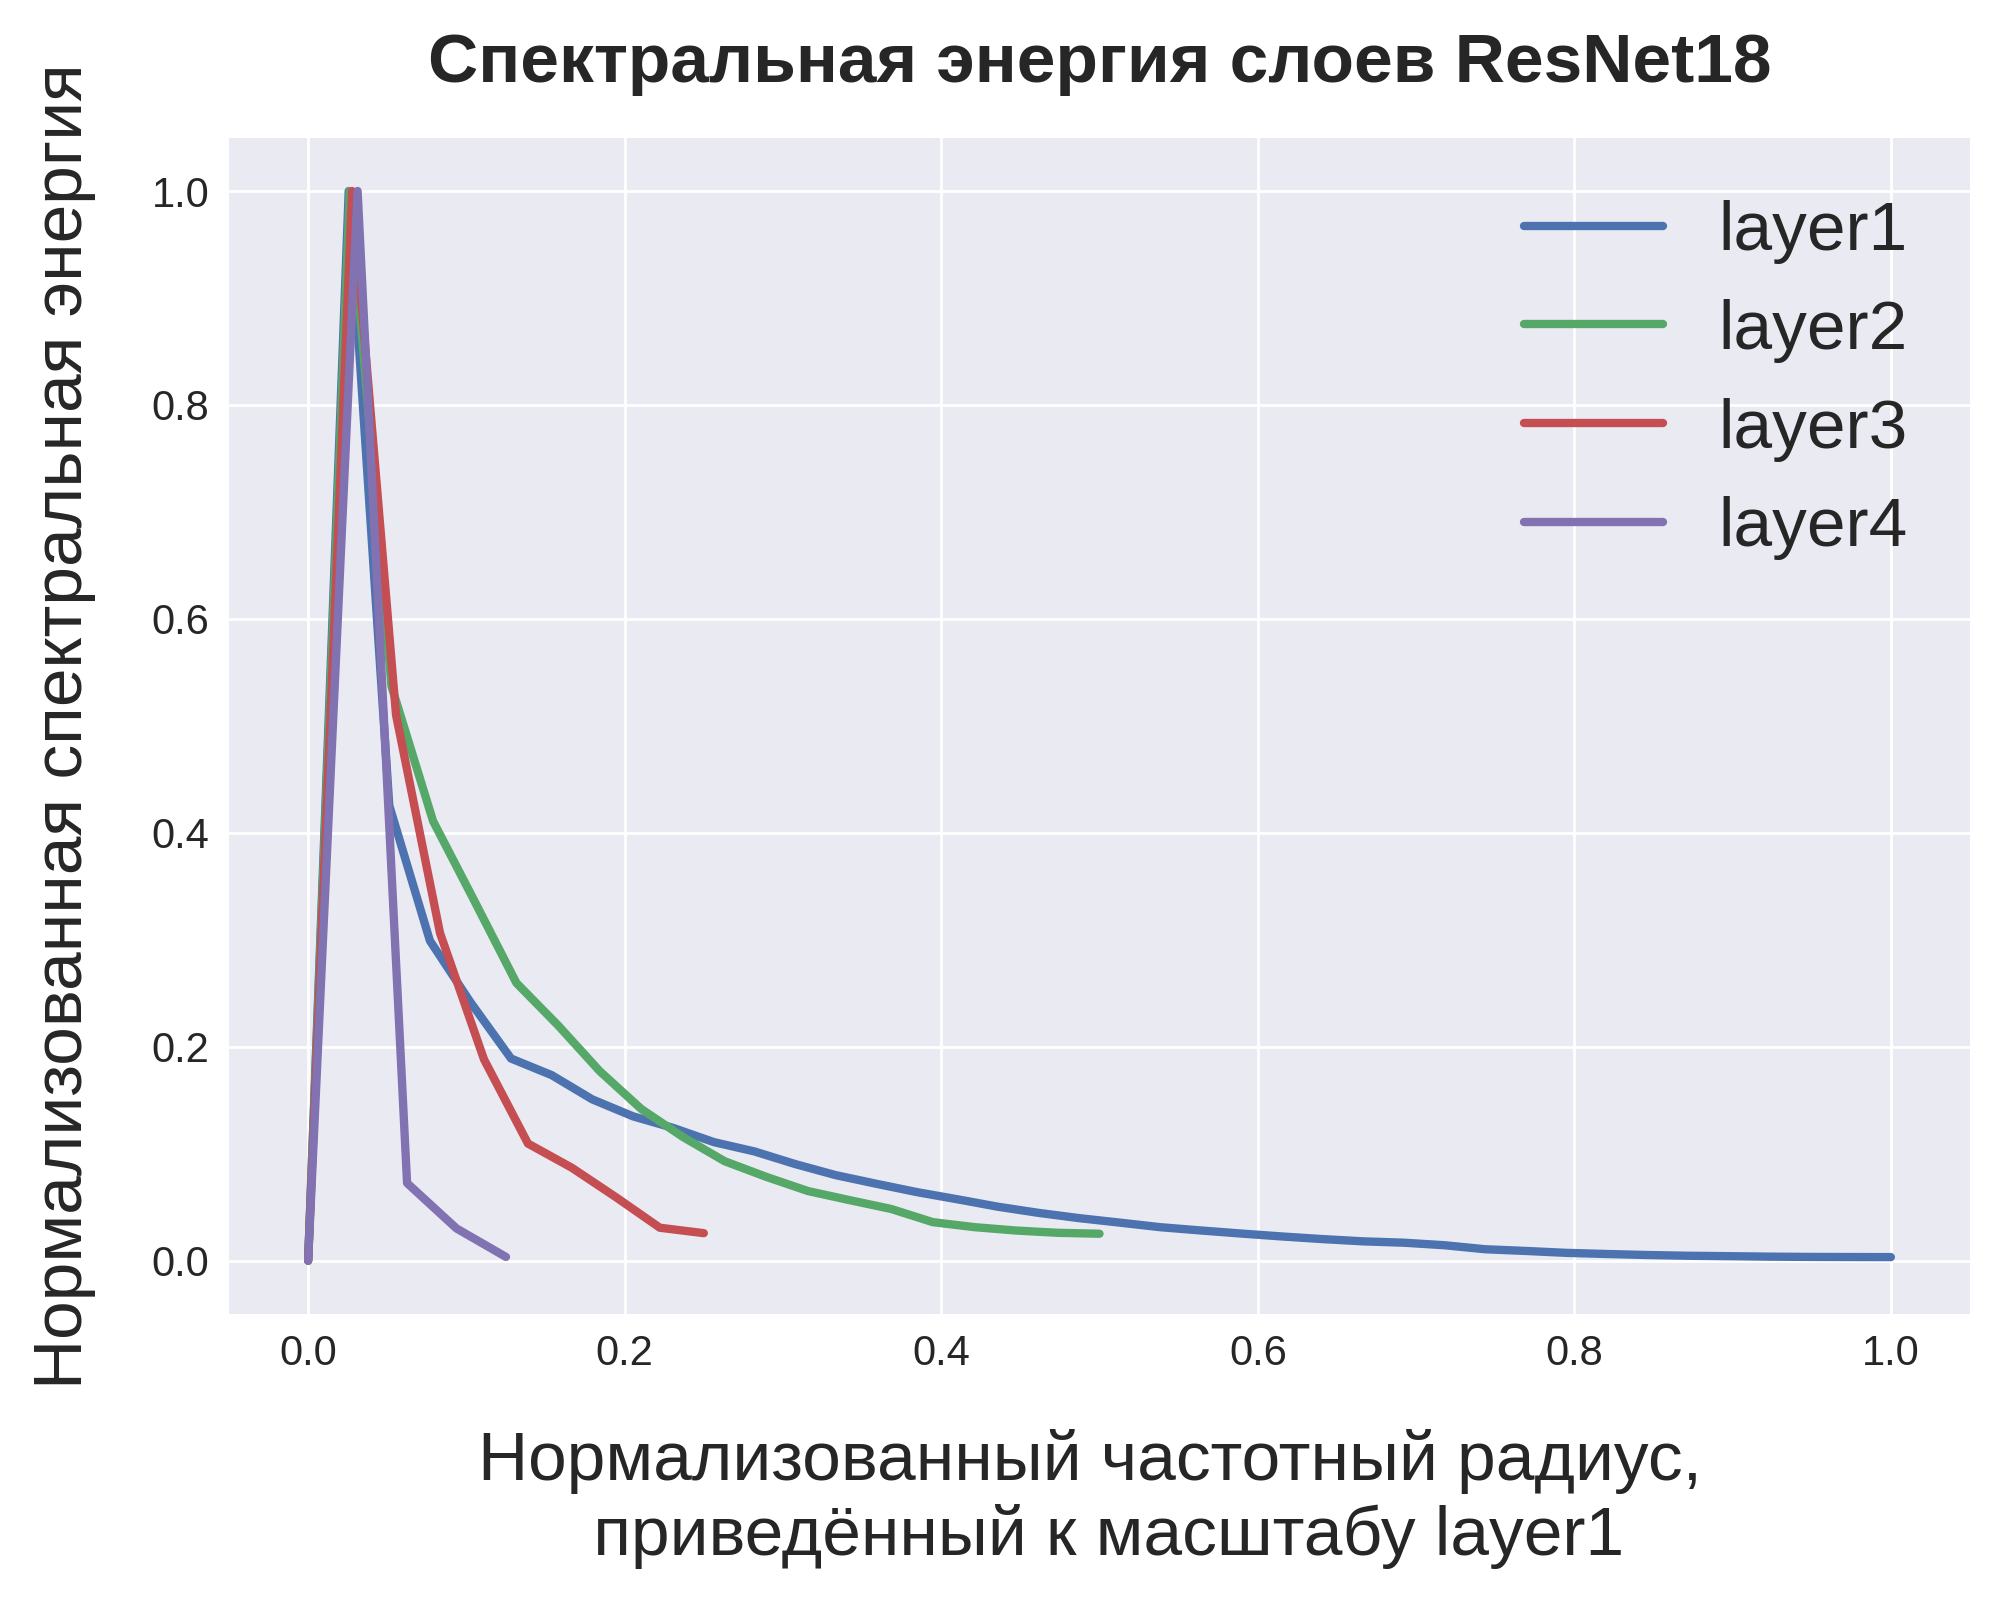
\includegraphics[width=0.8\textwidth]{images/compare/ResNet18.png} % Масштабируем до 80% ширины текста
    \caption{Изменение спектрального профиля по слоям ResNet18.} % Подпись
    \label{fig:ResNet18} % Метка для ссылки в тексте
\end{figure}

На Рис. \ref{fig:resnet_last_block} сравниваются спектры последнего блока у ResNet18, ResNet34, ResNet50 и ResNet101. Общая форма у всех моделей близкая: максимум находится в низкочастотной области, а доступный частотный диапазон после приведения к масштабу layer1 заметно ограничен. Значит, финальные представления всех вариантов ResNet имеют выраженный низкочастотный характер.

Различия между моделями всё же есть. У ResNet50 и ResNet101 хвост немного заметнее, чем у ResNet18 и ResNet34. Это согласуется с таблицей спектрального центроида: финальные значения у ResNet50/101 чуть выше, чем у ResNet18/34 (Таб. \ref{tab:SpectraCentr_metrics}). Но это различие не меняет основную картину. Внутри семейства ResNet глубина влияет на детали формы кривой, а не на сам тип финального спектрального профиля.

\begin{figure}[h]
    \centering % Центрируем изображение
    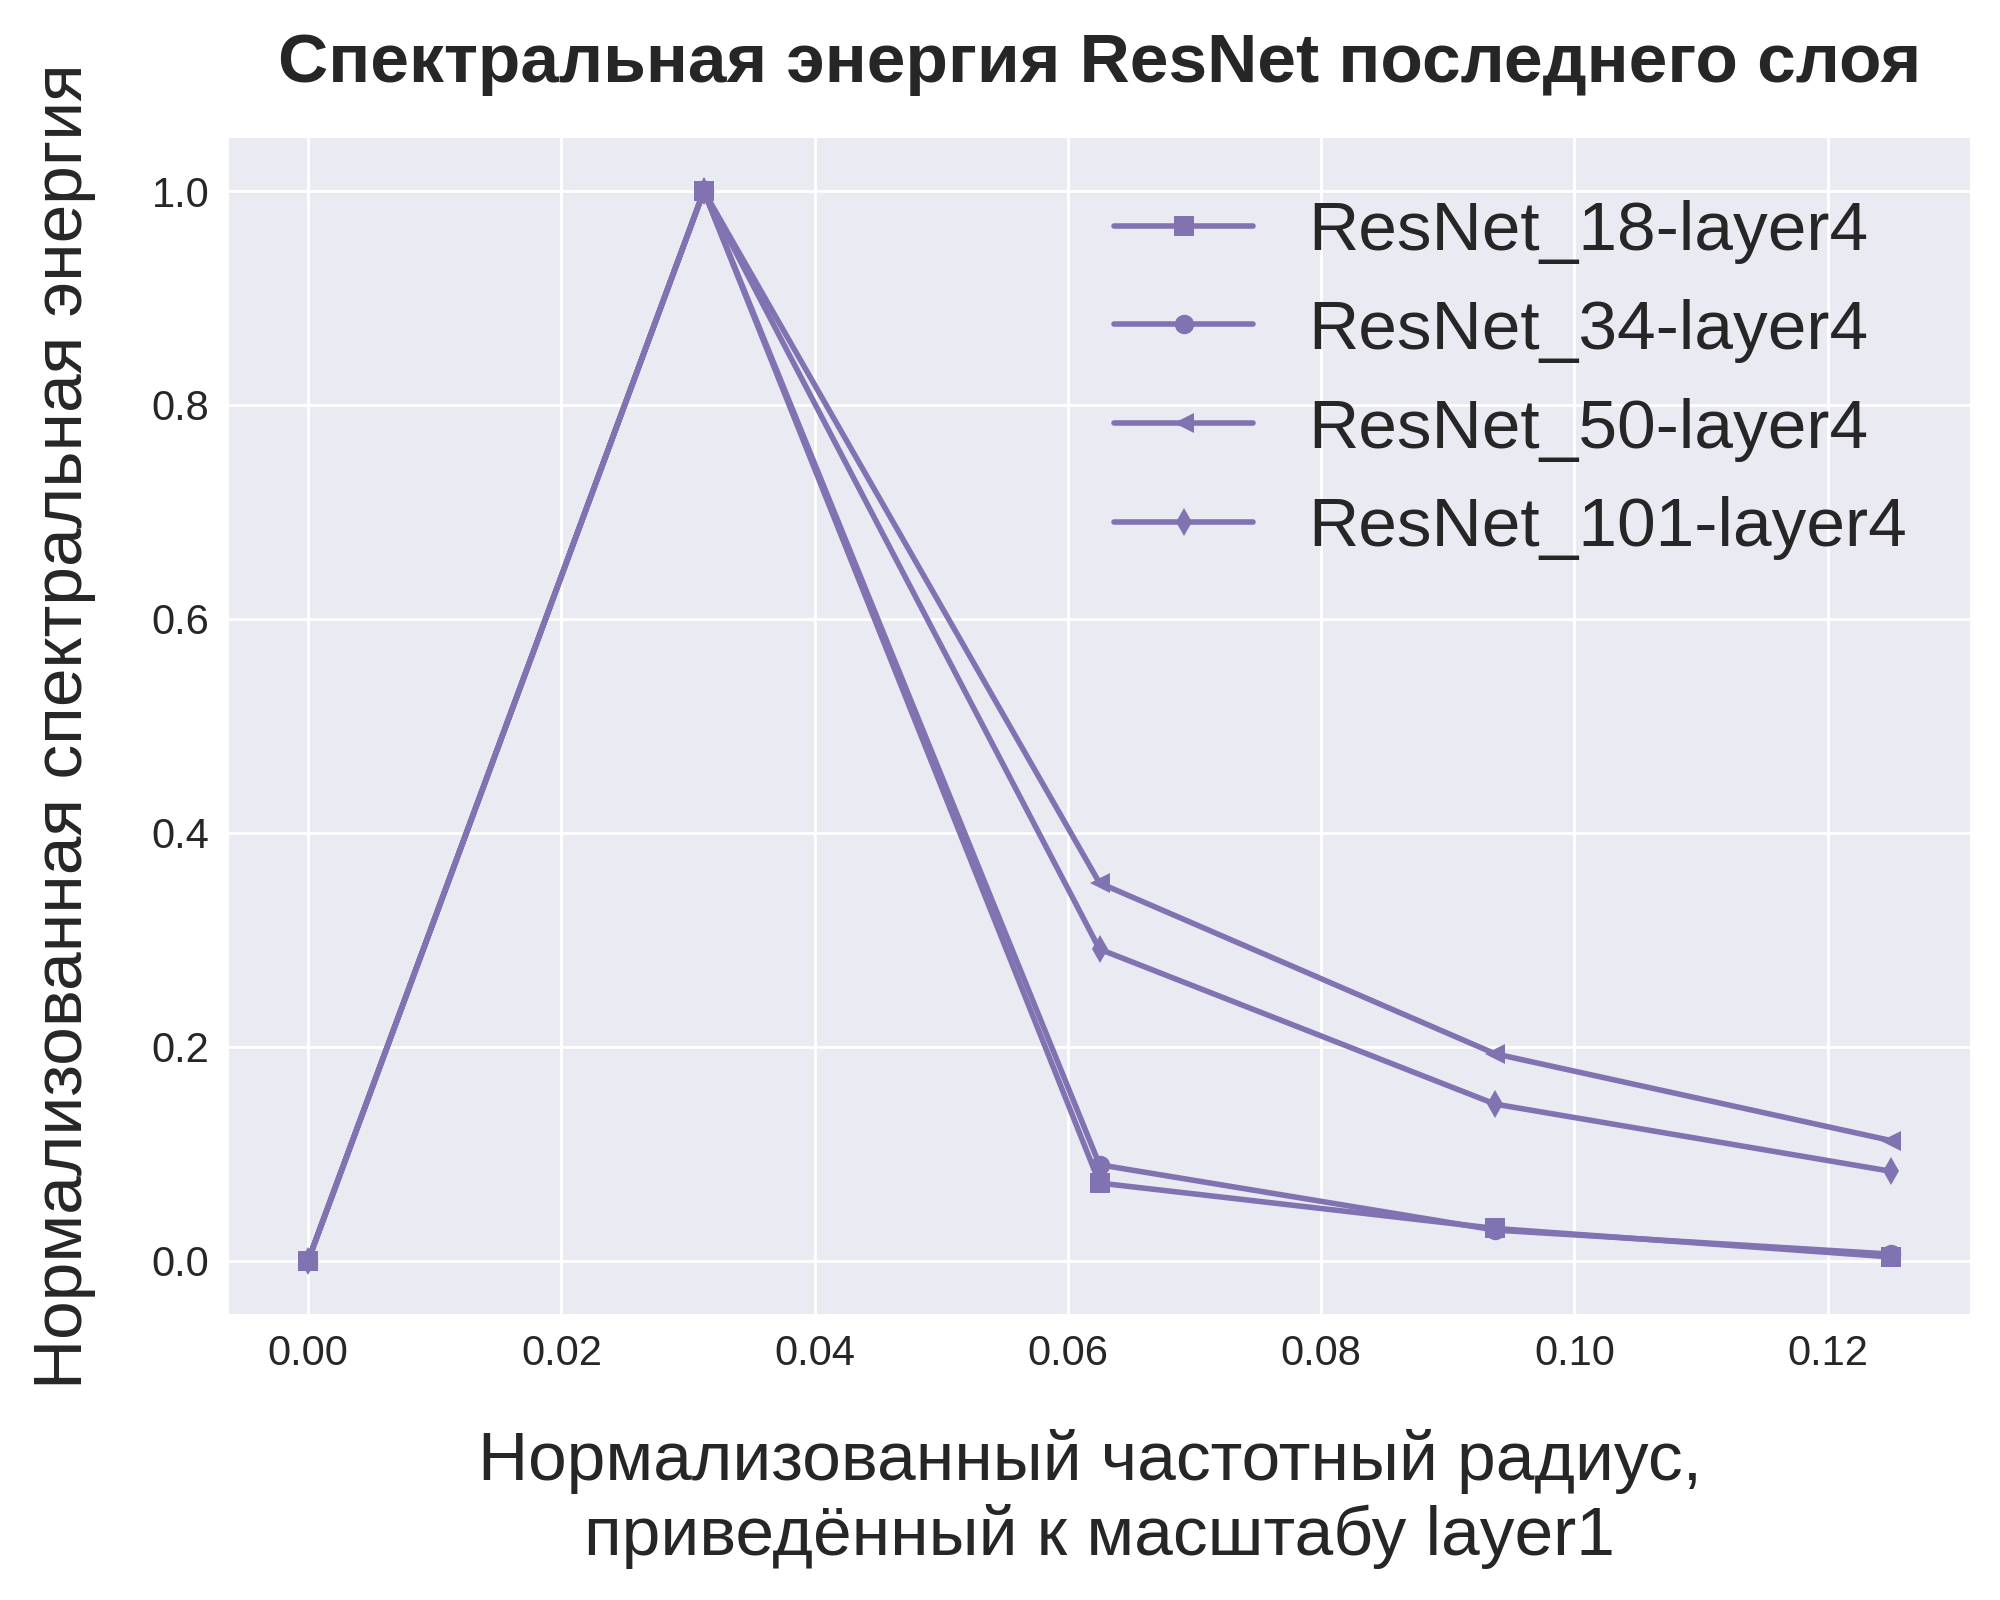
\includegraphics[width=0.8\textwidth]{images/compare/resnet_last_block.png} % Масштабируем до 80% ширины текста
    \caption{Сравнение спектров последних слоёв ResNet разной глубины.} % Подпись
    \label{fig:resnet_last_block} % Метка для ссылки в тексте
\end{figure}

\subsection{Динамика внутри ViT}

На Рис. \ref{fig:vit_l_16_imagenet_spectra} приведены спектральные кривые выбранных блоков ViT-L/16. По сравнению с ResNet поведение здесь другое. Не видно простого движения, при котором каждый следующий блок всё сильнее сжимает спектр к низким частотам. Напротив, поздние блоки ViT-L/16 сохраняют более длинный хвост в области средних и высоких частот. Особенно заметны block\_18 и block\_23: спад у них более пологий, а энергия на больших частотных радиусах остаётся заметной.

\begin{figure}[h]
    \centering % Центрируем изображение
    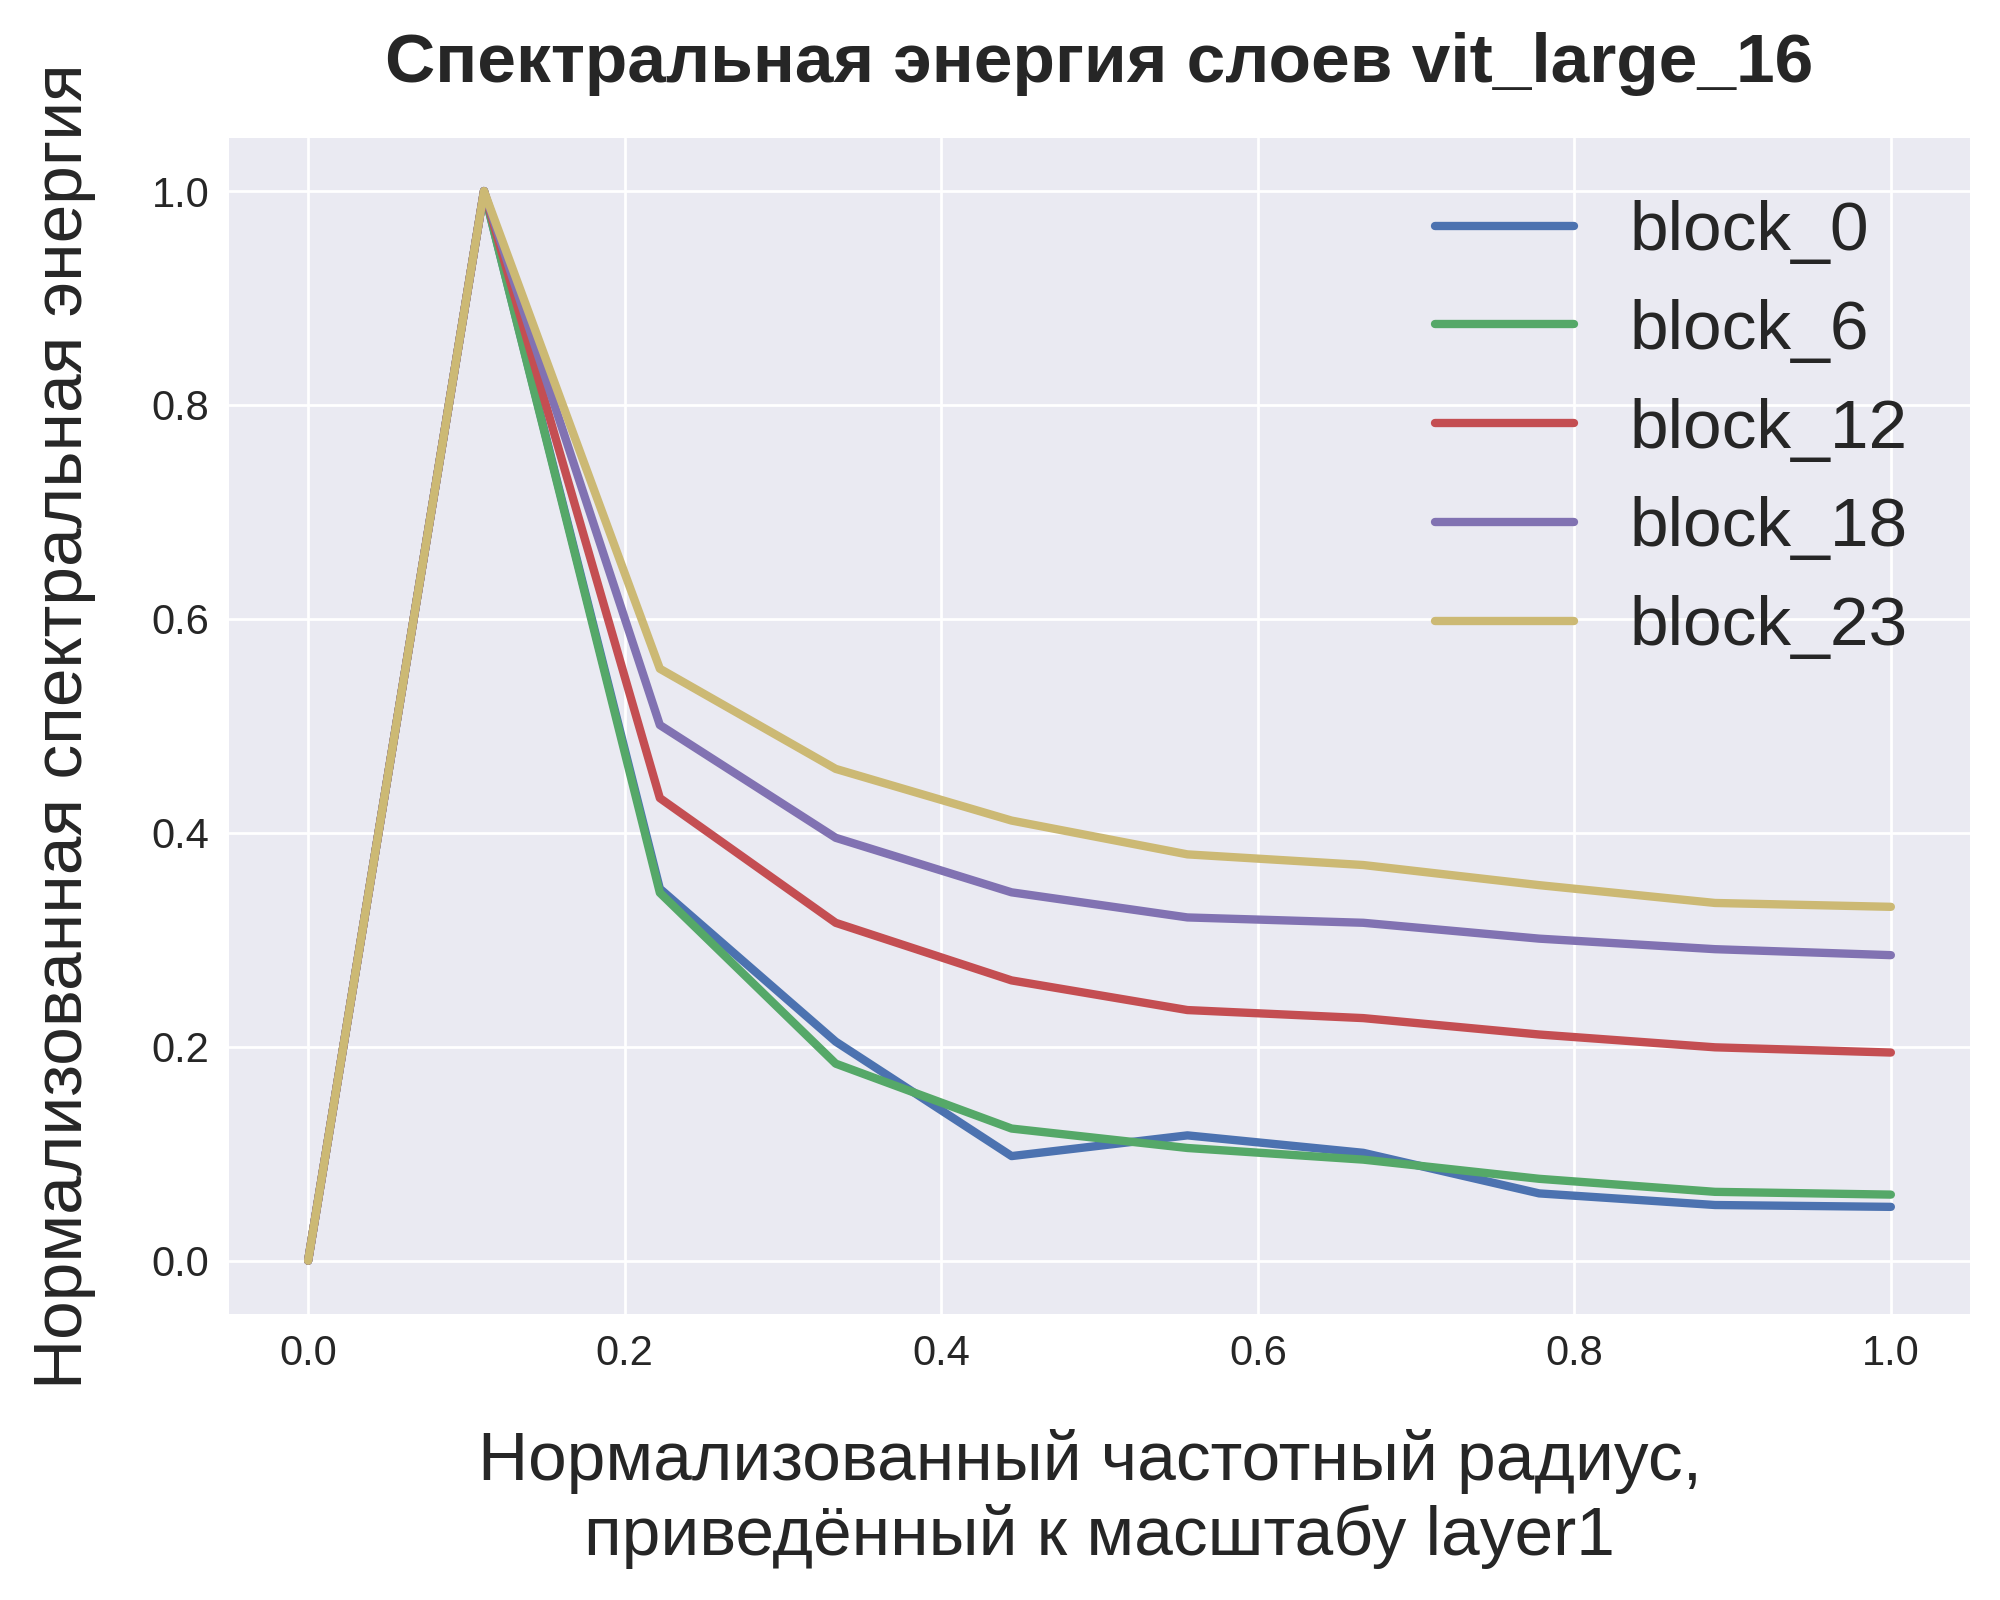
\includegraphics[width=0.8\textwidth]{images/compare/vit_l_16_imagenet_spectra.png} % Масштабируем до 80% ширины текста
    \caption{Изменение спектрального профиля по блокам ViT-L/16.} % Подпись
    \label{fig:vit_l_16_imagenet_spectra} % Метка для ссылки в тексте
\end{figure}

Причина такого отличия связана с устройством ViT. В ResNet пространственное разрешение уменьшается от стадии к стадии, и вместе с этим сужается набор частот, которые карта признаков может нести. В ViT последовательность патчей проходит через блоки при неизменной решётке. Преобразование задаётся вниманием, MLP-блоками и остаточными соединениями. Поэтому часть блоков может не только сглаживать токенные представления, но и усиливать различия между патчами.

Более широкий спектр на поздних блоках не стоит читать как прямое доказательство лучшего сохранения полезной семантики. График говорит о другом: в выбранном протоколе ViT-L/16 остаётся менее жёстко сжатым к низким частотам, чем CNN-представления. Что именно несёт эта энергия — полезные детали, особенности токенного кодирования или побочные вариации, — требует отдельной проверки. В рамках этой работы фиксируется сам факт: динамика ViT не похожа на последовательное подавление высоких частот.

Сравнение последних блоков моделей ViT (модификации Tiny, Small, Base и Large) представлено на Рис. \ref{fig:vit_block_last}. В отличие от ResNet, на финальном слое расхождения между этими конфигурациями становятся более очевидными. Для модели ViT-Large характерно наличие более протяженного «хвоста» на графике распределения, а также удержание большего объема относительной энергии в диапазоне средних частот.

\begin{figure}[h]
    \centering % Центрируем изображение
    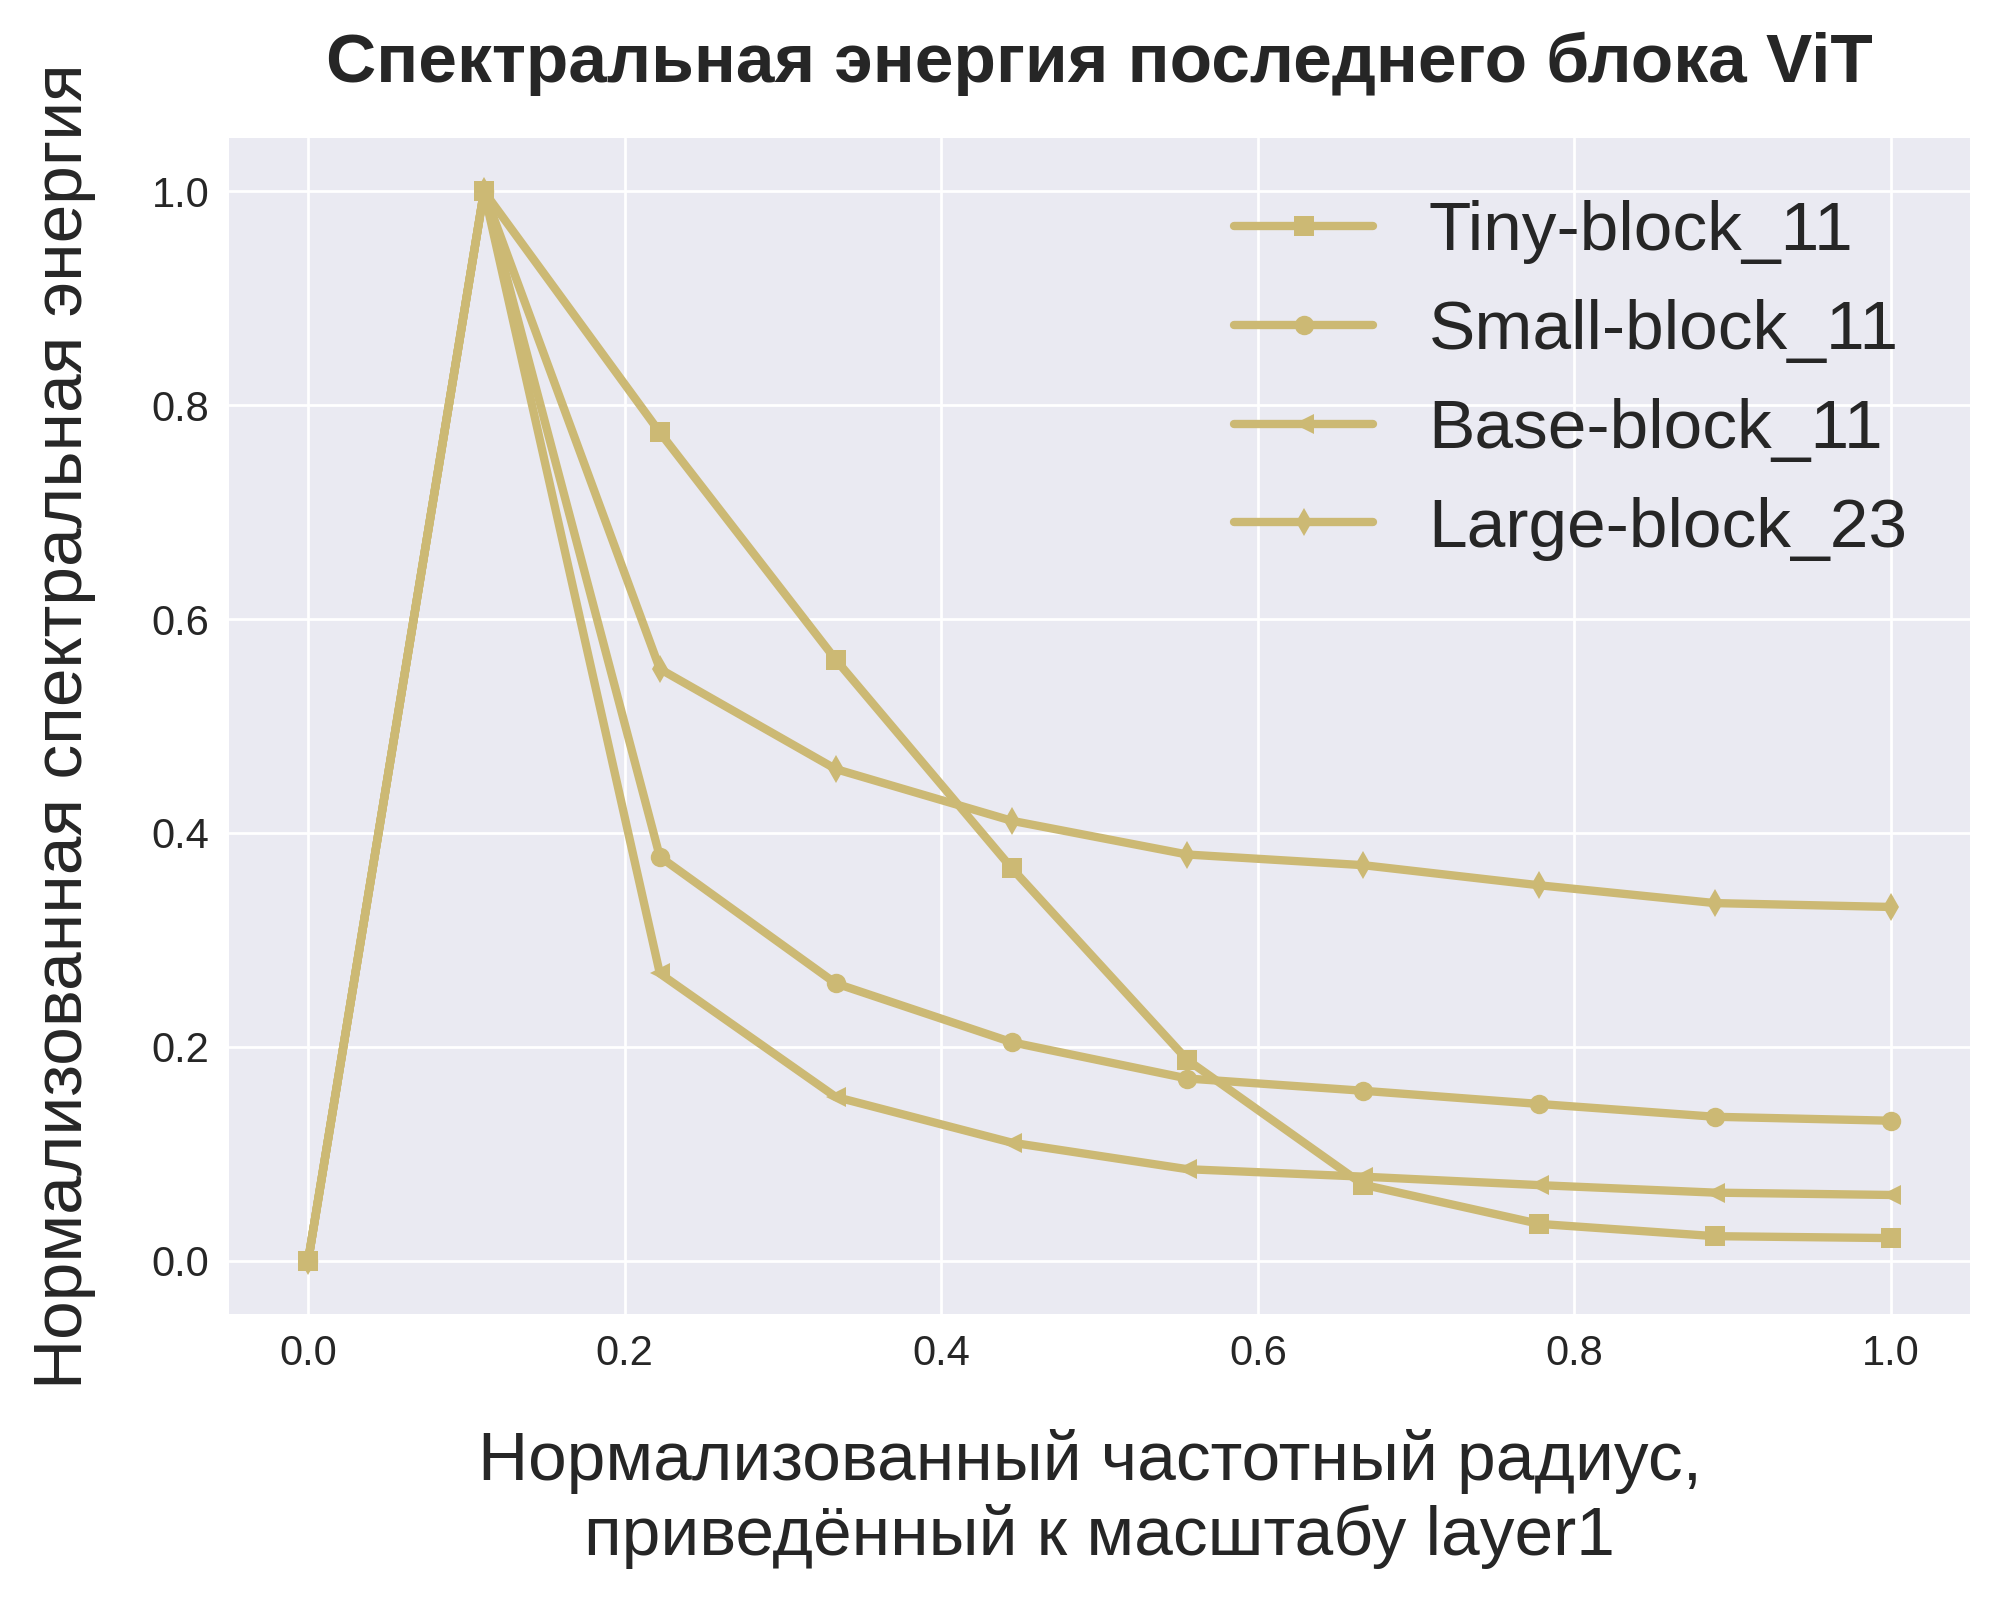
\includegraphics[width=0.8\textwidth]{images/compare/vit_block_last.png} % Масштабируем до 80% ширины текста
    \caption{Сравнение спектров последних слоёв ViT разного масштаба.} % Подпись
    \label{fig:vit_block_last} % Метка для ссылки в тексте
\end{figure}

На этом сравнении видно, что масштаб ViT отражается не только на числе параметров. Меняется и сам вид финального спектра. В данном эксперименте более крупная модель не приходит к более узкому низкочастотному профилю. Напротив, ViT-Large сохраняет более протяжённый хвост; это согласуется с повышенным центроидом large-модели в Таб. \ref{tab:SpectraCentr_metrics}. Поэтому внутри семейства ViT размер модели связан и с формой финального представления, а не только с вычислительной мощностью.

\subsection{Динамика внутри Swin}

На Рис. \ref{fig:swin_base} показана динамика выбранных блоков Swin-Base. Начальный блок даёт резкий пик около низких частот и сравнительно быстрый спад. Это похоже на сильную локальную агрегацию уже на раннем этапе обработки. Но далее картина не остаётся полностью простой: на промежуточных стадиях некоторые блоки имеют более широкий хвост и сохраняют заметную энергию в области средних частот. Вероятное объяснение — работа shifted window attention, где локальные окна чередуются со сдвинутыми окнами и дают обмен информацией между соседними областями изображения.

Поздний блок снова выглядит более низкочастотным. После перехода к последней иерархической стадии Swin приходит к более узкому спектральному диапазону, но путь к этому состоянию не повторяет ResNet один к одному. Swin здесь лучше описывать как архитектуру со смешанной динамикой: patch merging тянет представления к CNN-подобному сжатию, а оконное внимание даёт промежуточные перераспределения энергии.

\begin{figure}[h]
    \centering % Центрируем изображение
    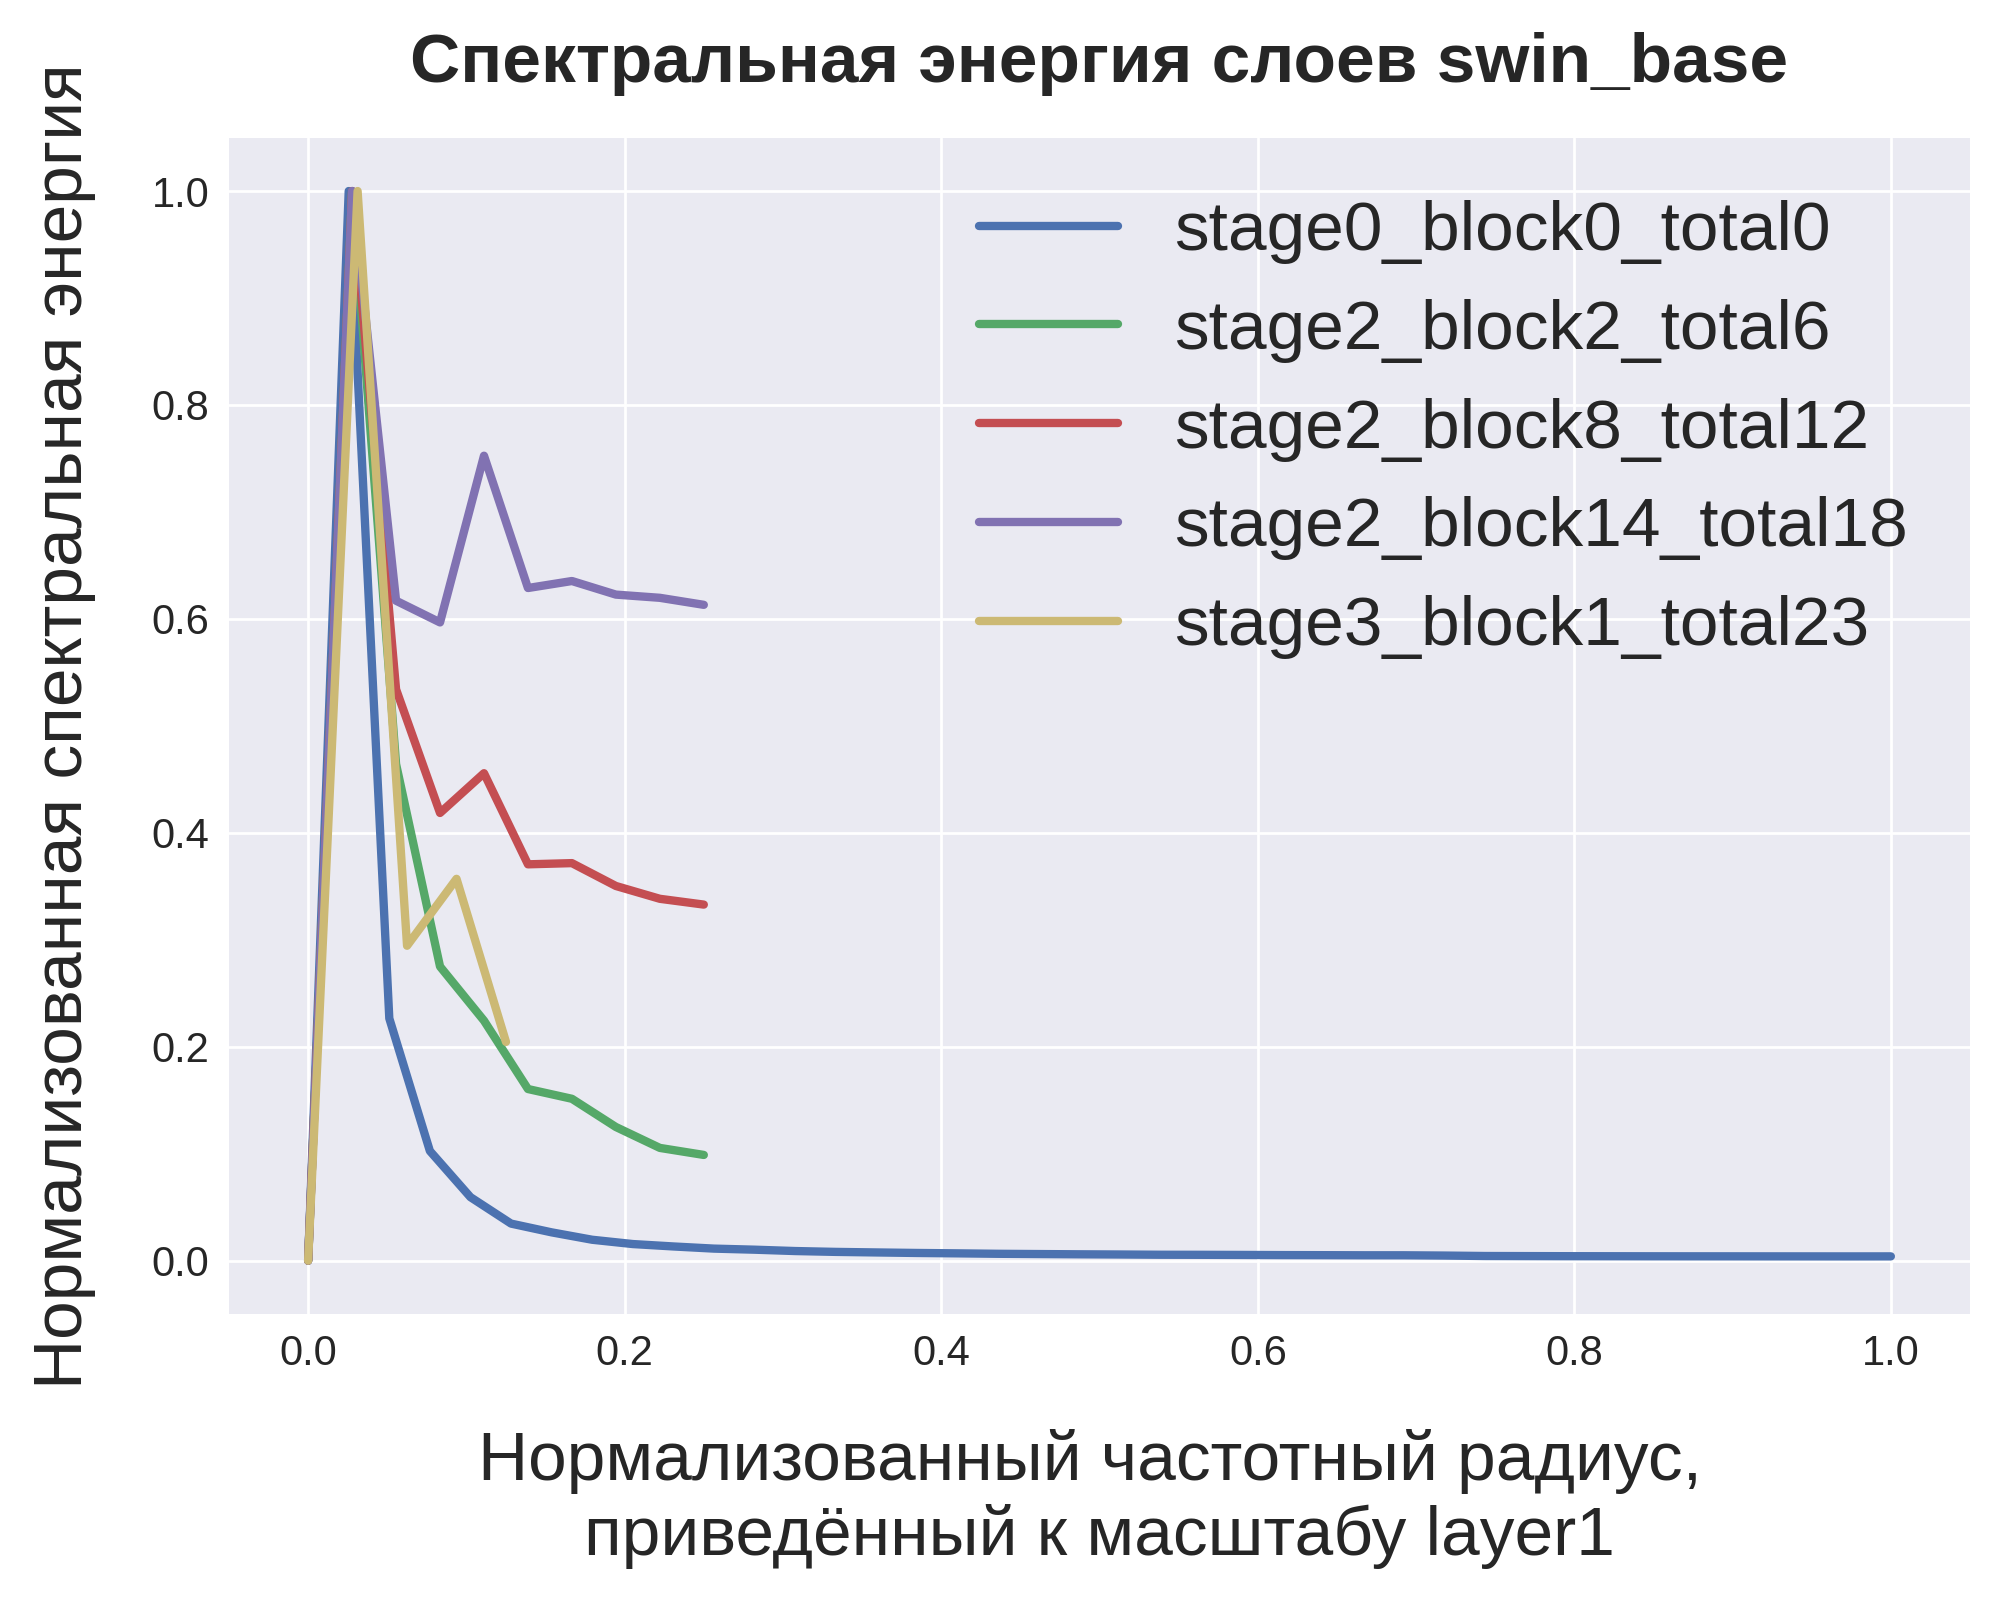
\includegraphics[width=0.8\textwidth]{images/compare/swin_base.png} % Масштабируем до 80% ширины текста
    \caption{Изменение спектрального профиля по блокам Swin-Base.} % Подпись
    \label{fig:swin_base} % Метка для ссылки в тексте
\end{figure}

На Рис. \ref{fig:swin_block_last} представлены спектры последних блоков Swin-Tiny, Swin-Small, Swin-Base и Swin-Large. Все кривые имеют общий максимум в низкочастотной области и достаточно близкую форму. Это отличает Swin от ViT: у ViT финальные спектры разных масштабов расходятся сильнее.

У Swin финальная стадия, судя по графику, стабилизируется архитектурной иерархией. Независимо от размера модели последние блоки приходят к сходному низкочастотному профилю. Локальное оконное внимание и объединение патчей не делают Swin обычной CNN, но в финальных представлениях они дают близкое направление спектрального сжатия.

\begin{figure}[h]
    \centering % Центрируем изображение
    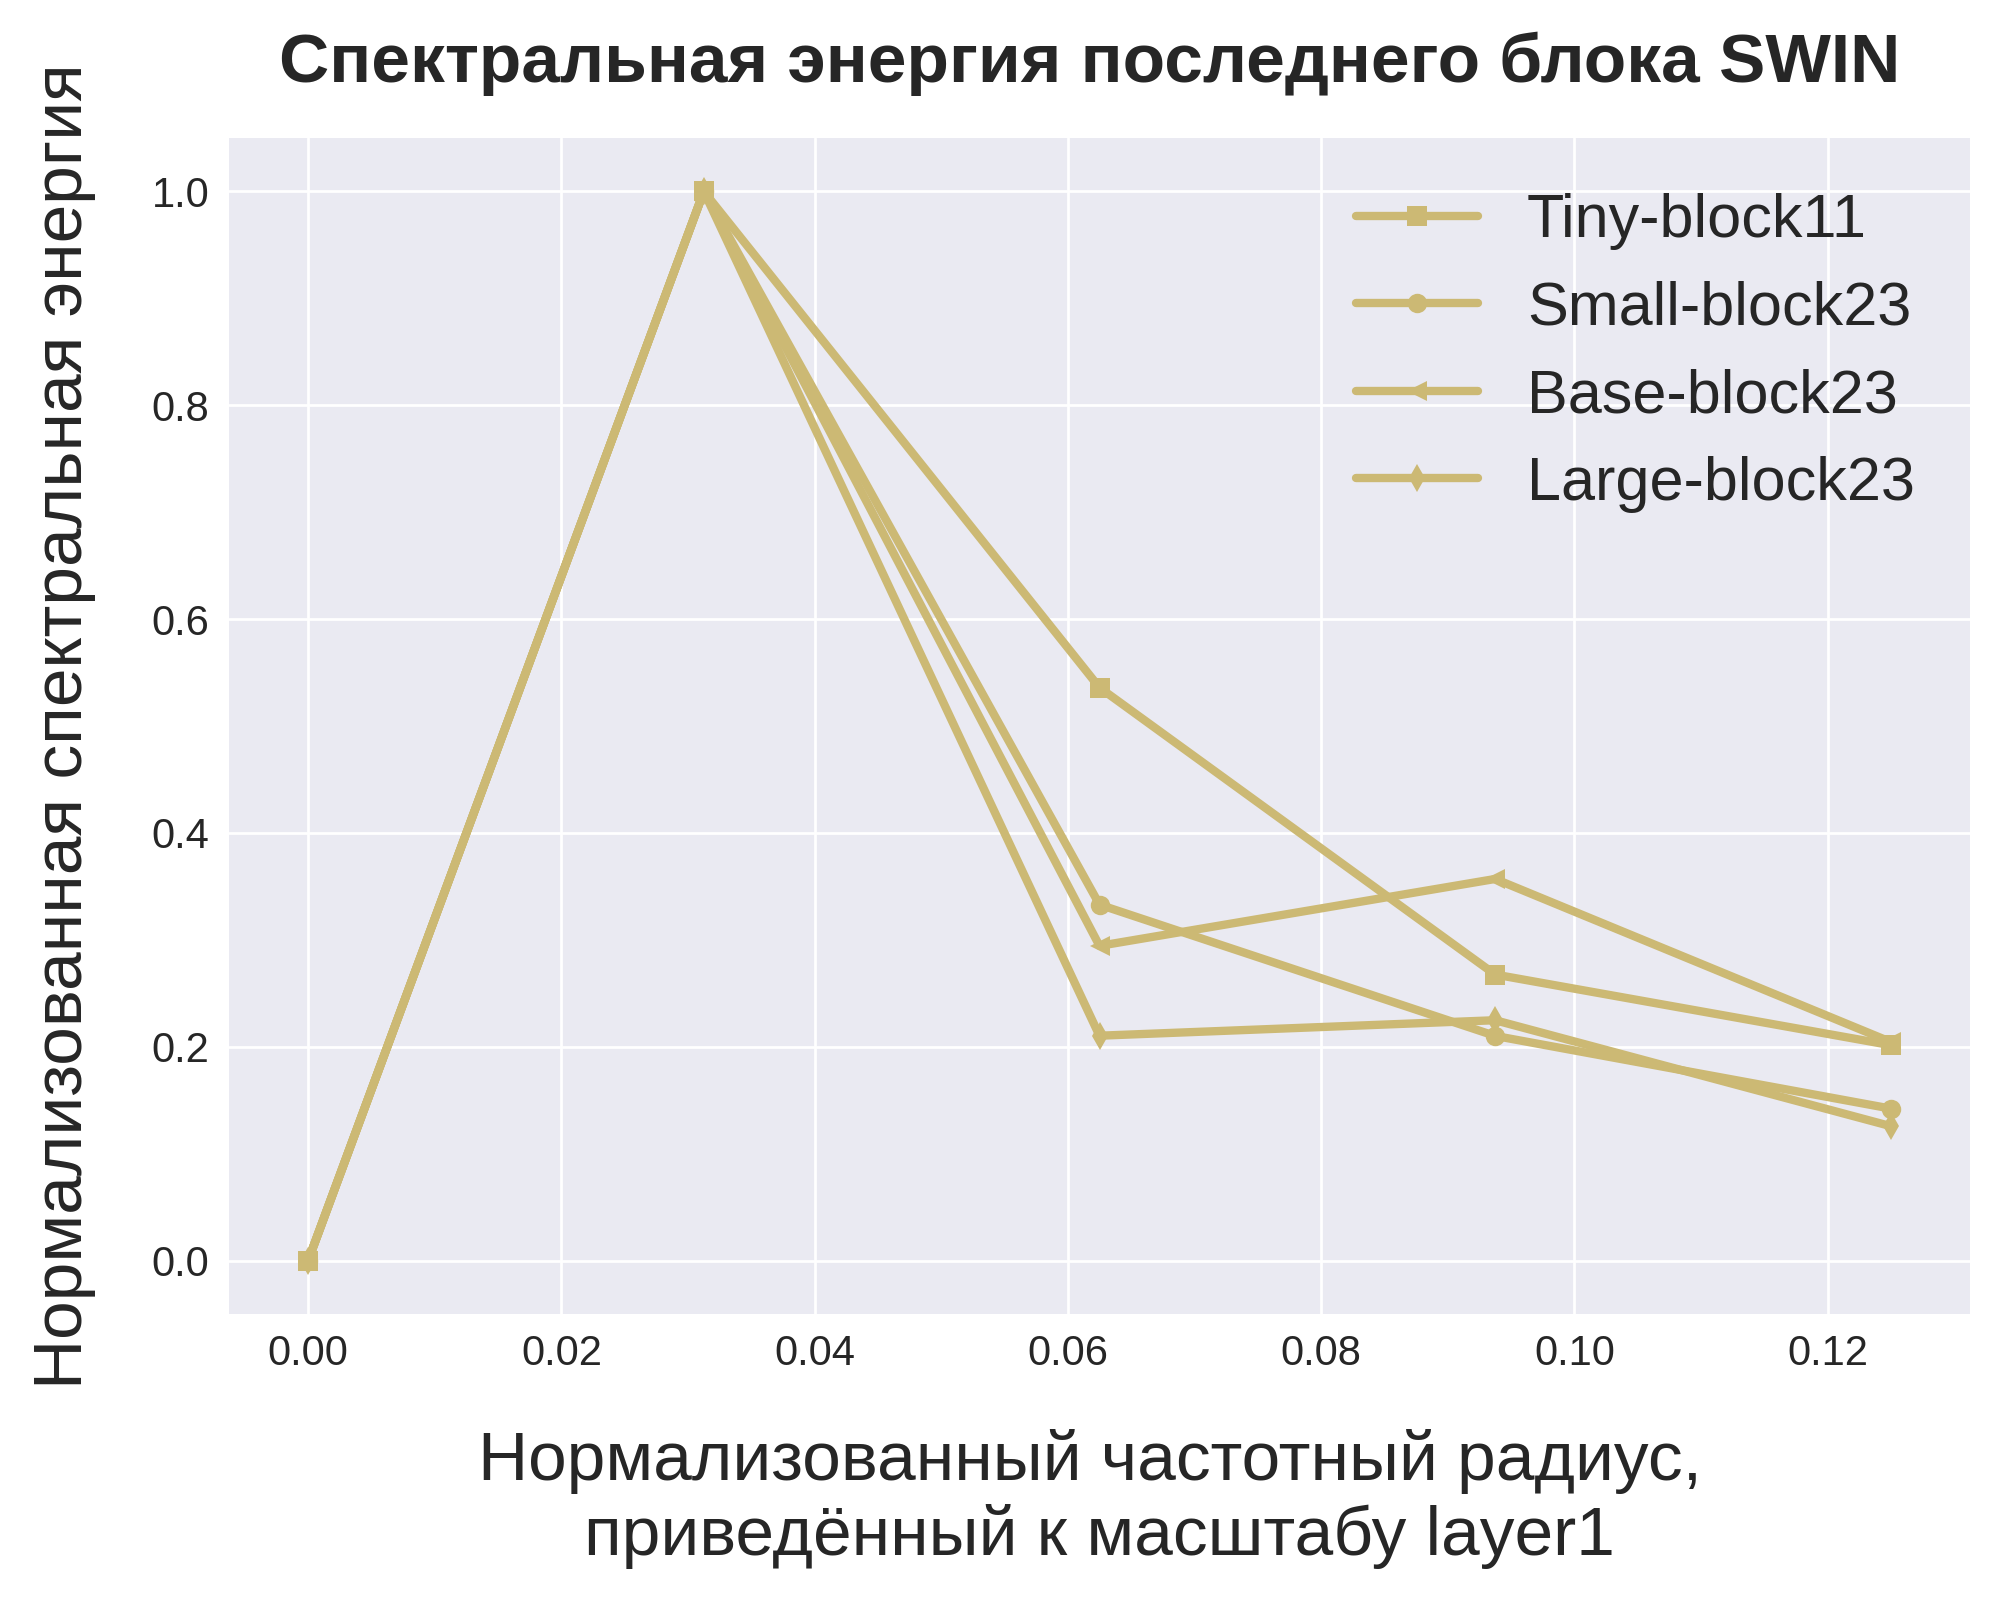
\includegraphics[width=0.8\textwidth]{images/compare/swin_block_last.png} % Масштабируем до 80% ширины текста
    \caption{Сравнение спектров последних слоёв Swin разного масштаба.} % Подпись
    \label{fig:swin_block_last} % Метка для ссылки в тексте
\end{figure}

\subsection{Межсемейственное сравнение архитектур}

На Рис. \ref{fig:compare_begin_block} показаны нормализованные радиальные спектры мощности для начальных уровней ResNet, ViT и Swin. У всех семейств максимум находится в области малых частотных радиусов. Значит, уже в начале обработки основная энергия признаков сосредоточена в низкочастотной области.

При этом кривые не совпадают. У ResNet хвост после основного пика выглядит более протяжённым: начальные свёрточные признаки ещё несут часть локальной текстурной информации. У ViT и Swin начальные представления формируются не как пиксельные карты признаков CNN, а через патчи и токены. Поэтому их спектральный профиль задаётся другой пространственной дискретизацией. На этом уровне различия между архитектурами ещё не максимальны, но видно, что каждая из них стартует с собственной формой распределения энергии.

\begin{figure}[h]
    \centering % Центрируем изображение
    
\includegraphics[width=0.8\textwidth]{images/compare/compare_begin_block.png} % Масштабируем до 80% ширины текста
    \caption{Сравнение радиальных спектров мощности начальных слоёв ResNet, ViT и Swin} % Подпись
    \label{fig:compare_begin_block} % Метка для ссылки в тексте
\end{figure}

На средних уровнях различия становятся заметнее. ResNet быстрее смещается к низкочастотной области: после пика энергия падает довольно резко, а вклад средних и высоких частот остаётся небольшим. Это хорошо согласуется с общей логикой CNN, где признаки постепенно агрегируются, рецептивное поле растёт, а пространственное разрешение уменьшается.

Сравнение средних слоёв на Рис. \ref{fig:compare_middle_block} показывает, что ViT не следует тому же сценарию. Его кривые имеют более протяжённый спад, то есть часть энергии сохраняется на средних частотах. Такая форма связана с тем, что ViT работает на решётке патчей без классического свёрточного downsampling между блоками.

Swin на этом графике ведёт себя наиболее неоднородно. Часть Swin-кривых убывает медленнее, чем ResNet, и сохраняет высокий уровень энергии в среднечастотной области. Поэтому для среднего уровня нельзя просто сказать, что Swin повторяет CNN. Скорее здесь проявляется его гибридная природа: иерархичность уже влияет на спектр, но оконное внимание и обмен между окнами дают более широкий частотный профиль.

\begin{figure}[h!]
    \centering % Центрируем изображение
    
\includegraphics[width=0.8\textwidth]{images/compare/compare_middle_block.png} % Масштабируем до 80% ширины текста
    \caption{Сравнение радиальных спектров мощности средних слоёв ResNet, ViT и Swin} % Подпись
    \label{fig:compare_middle_block} % Метка для ссылки в тексте
\end{figure}

На последних уровнях различия между семействами становятся наиболее заметными (Рис. \ref{fig:compare_last_block}). У ResNet спектры сужаются и концентрируются около малых частотных радиусов. Это соответствует финальному CNN-представлению, где локальные детали и текстурные изменения уже в основном подавлены. Дальше эту же картину подтверждают метрики: центроид у ResNet снижается, а доля низкочастотной энергии растёт.

Характер финальных кривых у архитектуры ViT принципиально иной. Ряд модификаций, в особенности масштабные конфигурации, демонстрируют выраженную хвостовую часть в среднечастотном спектре. Подобная картина контрастирует с жесткой фильтрацией низких частот, свойственной ResNet. Данное наблюдение согласуется со смещением спектрального центроида ViT в сторону более высоких значений на глубоких уровнях сети.

Финальный Swin по направлению изменения спектра ближе к CNN: диапазон становится уже, максимум остаётся около низких частот. Но полного совпадения с ResNet нет. У Swin сохраняются признаки трансформерной обработки, связанные с оконным вниманием и стадийной организацией. Поэтому его финальное поведение лучше описывать как промежуточное: низкочастотное по итоговому профилю, но сформированное другим механизмом.

\begin{figure}[h!]
    \centering % Центрируем изображение
    
\includegraphics[width=0.8\textwidth]{images/compare/compare_last_block.png} % Масштабируем до 80% ширины текста
    \caption{Сравнение радиальных спектров мощности последних слоёв ResNet, ViT и Swin} % Подпись
    \label{fig:compare_last_block} % Метка для ссылки в тексте
\end{figure}

По графикам видно, что трансформерные архитектуры не повторяют спектральную динамику CNN. ResNet даёт наиболее последовательное сжатие спектра, ViT показывает более свободное перераспределение энергии, а Swin оказывается между ними.

\section{Сводная интерпретация по метрикам}

Для численного сравнения использовались три показателя: спектральный центроид, доля низкочастотной энергии и скорость спектрального сжатия. Графики дают форму кривой, а метрики позволяют проверить те же наблюдения в компактном виде.

В Таб. \ref{tab:SpectraCentr_metrics} приведены значения спектрального центроида для моделей разных семейств. У ResNet картина самая ровная: центроид уменьшается от начальных уровней к глубоким во всех четырёх моделях. Для ResNet18 он падает с 0.176 до 0.035, для ResNet34 — с 0.169 до 0.036, для ResNet50 — с 0.203 до 0.049, для ResNet101 — с 0.206 до 0.046. Это численно подтверждает то, что было видно на графиках: по глубине ResNet сдвигает энергию к низким частотам.

Есть и небольшая деталь. У ResNet50 и ResNet101 начальный центроид выше, чем у ResNet18/34. Возможно, это связано с более широкой и сложной структурой bottleneck-блоков. Но к финальным уровням все модели приходят к близкому диапазону. Значит, более глубокая ResNet меняет траекторию сжатия, но итоговый низкочастотный характер остаётся общим для всего семейства.

\begin{table}[h]
\centering
\caption{Спектральный центроид различных архитектур} 
\label{tab:SpectraCentr_metrics}
\vspace{1ex} 
\begin{tabular}{llccc} % Добавлен один столбец 'l' слева
\toprule
\textbf{Архитектура} & \textbf{Тип} & \textbf{Начальные} & \textbf{Средние} & \textbf{Глубокие} \\
\midrule

% Первая группа строк
\multirow{4}{*}{CNN} & resnet18      & 0.176 & 0.121 & 0.035 \\
                     & resnet34      & 0.169 & 0.116 & 0.036 \\
                     & resnet50      & 0.203 & 0.128 & 0.049 \\
                     & resnet101     & 0.206 & 0.140 & 0.046 \\

\midrule

% Вторая группа строк                                                                                                       
\multirow{4}{*}{ViT} & tiny\_16      & 0.297 & 0.257 & 0.278 \\
                     & small\_16     & 0.312 & 0.419 & 0.346 \\
                     & base\_16      & 0.265 & 0.351 & 0.275 \\
                     & large\_16     & 0.275 & 0.385 & 0.437 \\
\midrule

% Третья группа строк
\multirow{4}{*}{Swin} & tiny       & 0.114 & 0.074 & 0.053 \\
                      & small      & 0.103 & 0.114 & 0.049 \\
                      & base       & 0.098 & 0.110 & 0.054 \\
                      & large      & 0.121 & 0.125 & 0.048 \\
\bottomrule
\end{tabular}
\end{table}

У ViT значения центроида выше и ведут себя менее регулярно. У ViT-large центроид растёт от 0.275 на начальном уровне до 0.437 на глубоком. У ViT-small и ViT-base максимум приходится на средний уровень: 0.419 и 0.351 соответственно. Такая динамика не похожа на устойчивое подавление средних и высоких частот. Скорее ViT перераспределяет энергию между блоками, а не просто сжимает её к низкочастотной области.

У Swin центроид в начале ниже, чем у ViT, а на глубоких блоках оказывается близок к ResNet. Финальные значения Swin лежат в диапазоне 0.048--0.054, тогда как у ResNet — 0.035--0.049. При этом средний уровень у Swin ведёт себя не полностью монотонно: у small, base и large центроид немного выше начального, у tiny — ниже. Это хорошо согласуется с графиками: Swin действительно приходит к низкочастотному финальному состоянию, но промежуточная динамика у него сложнее, чем у ResNet.

В Таб. \ref{tab:LowFrac_metrics} приведена доля низкочастотной энергии. Для CNN эта метрика растёт во всех моделях. У ResNet18 значение увеличивается с 17.3 до 31.2, у ResNet34 — с 17.8 до 31.2, у ResNet50 — с 16.6 до 30.1, у ResNet101 — с 16.3 до 30.3. Здесь центроид и доля низких частот дают согласованную картину: спектр ResNet по глубине сжимается, а низкочастотная область получает всё больший вес.

У ViT такой единой траектории нет. На начальных блоках доля низкочастотной энергии высокая: от 53.1 до 61.9. Но дальше каждая модель ведёт себя по-своему. У ViT-tiny она сначала растёт, затем падает. У ViT-small снижается на среднем уровне и частично восстанавливается на глубоком. У ViT-base после падения снова выходит на высокое значение. У ViT-large, наоборот, снижается почти монотонно — с 59.5 до 30.6. Это ещё раз показывает: ViT нельзя описать одной простой схемой низкочастотного накопления.

Высокая доля низкочастотной энергии у ViT не противоречит высокому центроиду. Эти показатели смотрят на распределение с разных сторон. Доля низких частот считает энергию ниже выбранного порога, а центроид учитывает всё распределение целиком. Поэтому возможна ситуация, когда значительная часть энергии находится у низких частот, но оставшаяся часть достаточно далеко растянута по частотной оси и поднимает центроид. Для ViT такая комбинация как раз и характерна.

У Swin доля низких частот к глубоким блокам растёт во всех вариантах. Начальные значения находятся около 21.5--22.6, глубокие — около 29.5--29.9. На среднем уровне изменения небольшие и не всегда направлены одинаково, но финальный переход к низкочастотному представлению сохраняется. В этом смысле Swin ближе к ResNet, чем к ViT, хотя степень и форма сжатия у него другие.

\begin{table}[h]
\centering
\caption{Доля низкочастотной энергии различных архитектур} 
\label{tab:LowFrac_metrics}
\vspace{1ex} 
\begin{tabular}{llccc} % Добавлен один столбец 'l' слева
\toprule
\textbf{Архитектура} & \textbf{Тип} & \textbf{Начальные} & \textbf{Средние} & \textbf{Глубокие} \\
\midrule

% Первая группа строк
\multirow{4}{*}{CNN} & resnet18      & 17.3 & 21.0 & 31.2 \\
                     & resnet34      & 17.8 & 21.6 & 31.2 \\
                     & resnet50      & 16.6 & 20.3 & 30.1 \\
                     & resnet101     & 16.3 & 19.2 & 30.3 \\

\midrule

% Вторая группа строк                                                                                                   
\multirow{4}{*}{ViT} & tiny\_16      & 55.6 & 63.5 & 44.7 \\
                     & small\_16     & 53.1 & 32.8 & 47.3 \\
                     & base\_16      & 61.9 & 47.0 & 62.5 \\
                     & large\_16     & 59.5 & 40.3 & 30.6 \\
\midrule

% Третья группа строк
\multirow{4}{*}{Swin} & tiny       & 21.8 & 25.9 & 29.6 \\
                      & small      & 22.4 & 22.2 & 29.9 \\
                      & base       & 22.6 & 22.6 & 29.5 \\
                      & large      & 21.5 & 21.3 & 29.9 \\
\bottomrule
\end{tabular}
\end{table}

Таб. \ref{tab:models_metrics} показывает скорость спектрального сжатия. У CNN все значения положительные и большие: от 0.46 до 0.51. Это самый выраженный режим сжатия среди трёх семейств. У ViT значения близки к нулю или отрицательны: от -0.0 до -0.12. По выбранной метрике это означает отсутствие устойчивого движения к низкочастотному представлению. У Swin значения положительные, но заметно меньше, чем у CNN: от 0.04 до 0.16. Значит, Swin всё же сжимает спектр к глубоким блокам, но делает это мягче.

\begin{table}[h]
\centering
\caption{Скорость спектрального сжатия} 
\label{tab:models_metrics}
\vspace{1ex} 

\begin{tabular}{ccccc} 
\toprule
\textbf{Архитектура} & \textbf{Tiny(18)} & \textbf{Small(34)} & \textbf{Base(50)} & \textbf{Large(101)} \\
\midrule
CNN    & 0.48 & 0.46  & 0.50  & 0.51 \\
ViT    & -0.0 & -0.05 & -0.02 & -0.12 \\
SWIN   & 0.16 & 0.07  & 0.04  & 0.12 \\
\bottomrule
\end{tabular}
\end{table}

Сопоставление трёх таблиц даёт общий вывод по метрикам. Тип архитектуры влияет на спектральную динамику сильнее, чем размер модели внутри одного семейства. Все ResNet демонстрируют сжатие, все Swin приходят к низкочастотному финальному профилю, но с меньшей скоростью, а ViT показывает наиболее нестабильную и немонотонную динамику. Это согласуется с визуальным анализом спектральных кривых.

\section{Обобщение экспериментальных результатов}

Совместный анализ графиков и таблиц показывает, что архитектуры различаются не только точностью или числом параметров. Они по-разному меняют частотный состав внутренних представлений. Это видно уже на уровне спектральных кривых, а затем подтверждается центроидом, долей низких частот и скоростью сжатия.

Для ResNet наблюдается самый понятный сценарий. Центроид падает, доля низкочастотной энергии растёт, скорость сжатия положительна во всех вариантах. Иначе говоря, ResNet последовательно переводит представления от более детальных пространственных признаков к сглаженным и семантически более крупным структурам. Это соответствует устройству CNN: свёртки, downsampling и рост рецептивного поля работают в одном направлении.

ViT ведёт себя иначе. Его центроид может расти на средних или поздних блоках, а доля низких частот меняется без единого шаблона. Это не случайная мелочь, а характерная особенность архитектуры: изображение обрабатывается как последовательность патчей, и блоки внимания вместе с MLP и residual-соединениями не обязаны давать монотонное спектральное сжатие. Поэтому ViT в данной постановке лучше описывать как модель с немонотонным перераспределением энергии по частотной оси.

Swin занимает промежуточное место. На глубоких блоках он приходит к низким значениям центроида и высокой доле низкочастотной энергии, то есть финально сближается с CNN. Но на средних уровнях у части моделей наблюдается менее прямой ход кривых и метрик. Возможно, это связано с тем, что Swin объединяет иерархию и patch merging с оконным вниманием. По результатам его нельзя назвать простой копией ResNet; это отдельный режим спектральной динамики.

Если сопоставить спектральные характеристики с точностью классификации, простой линейной зависимости не получается. Более сильное сжатие не всегда означает лучшую модель, а более широкий спектр не гарантирует более высокое качество. Спектральные метрики здесь работают иначе: они помогают понять, как устроены внутренние представления, но не заменяют accuracy.

Главный экспериментальный результат можно сформулировать так: ResNet даёт последовательное низкочастотное сжатие, ViT — немонотонное перераспределение спектральной энергии, Swin — промежуточную динамику с финальным смещением к низким частотам. Архитектура оказывается главным фактором, задающим форму этого поведения.


% \begin{table}[h]
% \centering
% \caption{Точность предсказаний} 
% \label{tab:models_metrics}
% \vspace{1ex} 

% \begin{tabular}{ссccc} 
% \toprule
% \textbf{Архитектура} & \textbf{Tiny(18)} & \textbf{Small(34)} & \textbf{Base(50)} & \textbf{Large(101)} \\
% \midrule
% CNN    &  79.04  &  85.36  &  92.89  &  93.96 \\
% ViT    &  82.10  &  87.96  &  92.02  &  92.28 \\
% SWIN   &  88.19  &  91.59  &  92.25  &  93.03 \\
% \bottomrule
% \end{tabular}
% \end{table}

\chapter{Заключение}

В работе были рассмотрены спектральные характеристики внутренних представлений трёх семейств моделей компьютерного зрения: ResNet, ViT и Swin. В фокусе исследования находился не только итоговый класс на выходе модели, а то, что происходит внутри: как по слоям меняется распределение энергии признаков по пространственным частотам. Иначе говоря, сохраняет ли модель более детальную, высокочастотную структуру или постепенно переводит представления в более сглаженный низкочастотный вид.

Для этого был собран единый протокол спектрального анализа. В случае ResNet анализировались карты признаков основных блоков. Для ViT последовательность токенов переводилась обратно в двумерную решётку патчей. Для Swin учитывалась его стадийная структура и изменение пространственного разрешения между уровнями. После получения представлений строился спектр мощности, затем выполнялось радиальное усреднение и нормализация. По полученным кривым рассчитывались три численные характеристики: спектральный центроид, доля низкочастотной энергии и скорость спектрального сжатия.

В начале исследования были сформулированы четыре гипотезы. Они и задавали логику экспериментальной части.

Первая гипотеза относилась к свёрточным сетям. Предполагалось, что ResNet по мере продвижения к глубоким блокам будет сдвигать спектр представлений в область низких частот. Эта гипотеза подтвердилась. Во всех рассмотренных моделях ResNet спектральный центроид снижается от ранних уровней к поздним, а доля низкочастотной энергии, наоборот, растёт. По числам это видно достаточно ясно: центроид меняется примерно от диапазона 0.17--0.21 на начальных блоках до 0.035--0.049 на глубоких. Доля низкочастотной энергии увеличивается примерно с 16--18\% до 30--31\%. Скорость сжатия у CNN также остаётся положительной и находится в диапазоне 0.46--0.51. По сути, ResNet ведёт себя как и ожидалось от иерархической свёрточной архитектуры: локальные детали на ранних уровнях постепенно уступают место более крупным и агрегированным признакам.

Вторая гипотеза касалась ViT. Я исходил из того, что Vision Transformer не обязан повторять поведение CNN, потому что он работает не со свёрточной пирамидой признаков, а с последовательностью патчевых токенов. Результаты это подтвердили. У ViT спектральный центроид не показывает устойчивого снижения. В отдельных моделях он, наоборот, растёт на средних или поздних блоках. Например, у ViT-large центроид увеличивается с 0.275 на начальном уровне до 0.437 на глубоком. С долей низкочастотной энергии картина тоже не такая ровная: у ViT-large она падает с 59.5\% до 30.6\%, а у ViT-base остаётся высокой даже на глубоких блоках. Значит, частотная динамика ViT устроена сложнее, чем простое движение к низким частотам. На неё, вероятно, одновременно влияют attention, MLP-блоки, нормализации и остаточные связи.

Третья гипотеза была связана со Swin Transformer. Предполагалось, что из-за patch merging и иерархической структуры Swin в конце будет приходить к более низкочастотным представлениям, но при этом его промежуточное поведение не обязано быть таким же прямым, как у CNN. Эта гипотеза подтвердилась, но с уточнением. На глубоких блоках Swin действительно даёт низкие значения центроида — примерно 0.048--0.054, а доля низкочастотной энергии выходит на уровень 29--30\%. Это близко к финальным значениям ResNet. Но на средних уровнях у части моделей центроид немного возрастает относительно начального уровня. Значит, Swin нельзя просто назвать ``CNN с вниманием''. Он скорее сочетает два механизма: иерархическое сжатие, похожее на CNN, и более сложное перераспределение признаков внутри трансформерных блоков.

Четвёртая гипотеза проверяла связь спектральных характеристик с точностью классификации. Здесь ожидалось, что прямой линейной зависимости не будет. Так и получилось. ResNet показывает самое выраженное спектральное сжатие и при этом достигает высокой точности в крупных вариантах. ViT сохраняет более широкий и местами немонотонный спектральный профиль, но это не приводит к автоматическому превосходству над лучшими ResNet и Swin. Swin, в свою очередь, хорошо работает на малых и средних масштабах, совмещая умеренное сжатие спектра с иерархической организацией признаков. Поэтому спектральные метрики полезны прежде всего как инструмент интерпретации. Они объясняют, как устроены представления, но не заменяют accuracy и не дают полного ответа о качестве модели.

Общий результат можно сформулировать так: архитектура заметно влияет на спектральную динамику внутренних представлений. ResNet даёт наиболее последовательное низкочастотное сжатие. ViT ведёт себя немонотонно: спектральная энергия может перераспределяться в сторону средних и более высоких частот даже на поздних блоках. Swin занимает промежуточную позицию: на финальных стадиях он становится близок к CNN по низкочастотному профилю, но по пути к этому состоянию демонстрирует более сложную динамику.

Практический смысл полученных результатов состоит в том, что предложенный протокол можно использовать для диагностики моделей компьютерного зрения. Он показывает, насколько быстро архитектура теряет или сохраняет частотное разнообразие признаков. Для задач, где мелкие локальные детали действительно несут полезную информацию, такой анализ может быть особенно полезен. Речь, например, о медицинских снимках, спутниковых изображениях, дефектоскопии, текстурах и мелких объектах.

У работы есть и ограничения. Спектральная энергия не равна информации в строгом смысле. Она не показывает напрямую, полезен ли конкретный частотный диапазон для классификации, не учитывает фазу спектра и не заменяет проверку качества на целевой задаче. Отдельное ограничение связано с ViT и Swin: перевод токенов в двумерную решётку нужен для сравнения с CNN, но такая решётка не является полной копией классической карты признаков. Токен уже содержит агрегированную информацию о патче, и это надо учитывать при интерпретации.

Дальше эту работу можно развивать в нескольких направлениях. Во-первых, полезно посмотреть, как спектральные метрики меняются не только у готовых моделей, но и в процессе обучения. Во-вторых, можно проверить связь спектрального профиля с устойчивостью к шуму и состязательным возмущениям. Ещё одно направление — перенести анализ на детекцию и сегментацию, где пространственная локализация признаков имеет большее значение, чем в обычной классификации. Наконец, на основе таких измерений можно пробовать строить регуляризаторы, которые будут контролировать сохранение или подавление отдельных частотных диапазонов.

\printbib  %Литература

% Следующие строки необходимо раскомментировать, а предыдущую закомментировать, если используется inline-библиография.
%\begin{thebibliography}{99}
%    \bibitem{langmuir26}
%        H. Mott-Smith, I. Langmuir. ``The theory of collectors in gaseous discharges''. \emph{Phys. Rev.} \textbf{28} (1926)
%\end{thebibliography}

\end{document}